%%%%%%%%%%%%%%%%%%%%%%%%%%%%%%%%%%%%%%%%%%%%%%%%%%%%%%%%%%%%%%%%%%%%%%%%%
%                                                                       %
% ustthesis_test.tex: A template file for usage with ustthesis.cls      %
%                                                                       %
%%%%%%%%%%%%%%%%%%%%%%%%%%%%%%%%%%%%%%%%%%%%%%%%%%%%%%%%%%%%%%%%%%%%%%%%%

\documentclass{ustthesis}

\usepackage{mathpazo,amsmath,amssymb,epsfig,enumerate,bbm,calc,color,ifthen,capt-of}
\usepackage{algorithm}
\usepackage[noend]{algorithmic}
\usepackage[center]{subfigure}
\usepackage{graphicx}
\usepackage{epstopdf}
\usepackage{booktabs}
\usepackage{threeparttable}
\newtheorem{proof}{Proof}
\usepackage{cite}
\usepackage{hyperref} % for better viewing experience  -- added by alan
\usepackage[margin=25mm,textheight=247mm,textwidth=145mm]{geometry}

% Alan: begin the font trial
% Euler for math | Palatino for rm | Helvetica for ss | Courier for tt
\renewcommand{\rmdefault}{ppl} % rm
%\linespread{1.05}        % Palatino needs more leading
\usepackage[scaled]{helvet} % ss
\usepackage{courier} % tt
%\usepackage{euler} % math
\usepackage{eulervm} % a better implementation of the euler package (not in gwTeX)
\normalfont
\usepackage[T1]{fontenc}
% Alan: end the font trial

\newcommand{\red}[1]{#1}
\newcommand{\tab}[1]{\hspace{3mm}}

% \usepackage{latexsym}
    % Use the "latexsym" package when encountering the following error:
    %   ! LaTeX Error: Command \??? not provided in base LaTeX2e.
\usepackage{epsf}
    % Use the "epsf" package for including EPS files.

%%%%%%%%%%%%%%%%%%%%%%%%%%%%%%%%%%%%%%%%%%%%%%%%%%%%%%%%%%%%%%%%%%%%%%%%%
%                                                                       %
% Preambles. DO NOT ERASE THEM. Change to suite your particular purpose.%
%                                                                       %
%%%%%%%%%%%%%%%%%%%%%%%%%%%%%%%%%%%%%%%%%%%%%%%%%%%%%%%%%%%%%%%%%%%%%%%%%

\title{	
	Import Exchange Rate Pass-through and Credit Constraints: Evidence from China}  % Title of the thesis.
\author{Lingfei Lu}     % Author of the thesis.
\degree{\MPhil}             % Degree for which the thesis is.
%% or
%\degree{\PhD}              % Degree for which the thesis is.
\subject{Economics}      % Subject of the Degree.
\department{Economics}       % Department to which the thesis
                    % is submitted.
\advisor{Assocciate Professor Yao Amber LI}     % Supervisor.
\depthead{Professor David Edward COOK}    % department head.
\defencedate{2022}{07}{28}      % \defencedate{year}{month}{day}.

% NOTE:
%   According to the sample shown in the guidelines, page number is
%   placed below the bottom margin.  However, if the author prefers
%   the page number to be printed above the bottom margin, please
%   activate the following command.

% \PNumberAboveBottomMargin

\begin{document}

%%%%%%%%%%%%%%%%%%%%%%%%%%%%%%%%%%%%%%%%%%%%%%%%%%%%%%%%%%%%%%%%%%%%%%%%%
%                                                                       %
% Now the actual Thesis. The order of output MUST be followed:          %
%                                                                       %
%    1) TITLEPAGE                                                       %
%                                                                       %
% The \maketitle command generates the Title page as well as the        %
% Signature page.                                                       %
%                                                                       %
%%%%%%%%%%%%%%%%%%%%%%%%%%%%%%%%%%%%%%%%%%%%%%%%%%%%%%%%%%%%%%%%%%%%%%%%%

\maketitle

%%%%%%%%%%%%%%%%%%%%%%%%%%%%%%%%%%%%%%%%%%%%%%%%%%%%%%%%%%%%%%%%%%%%%%%%%
%                                                                       %
%     2) DEDICATION (Optional)                                          %
%                                                                       %
% The \dedication and \enddedication commands are optional. If          %
% specified it generates a page for dedication.                         %
%
%%%%%%%%%%%%%%%%%%%%%%%%%%%%%%%%%%%%%%%%%%%%%%%%%%%%%%%%%%%%%%%%%%%%%%%%%

% \dedication
% This is an optional section.
% \enddedication

%%%%%%%%%%%%%%%%%%%%%%%%%%%%%%%%%%%%%%%%%%%%%%%%%%%%%%%%%%%%%%%%%%%%%%%%%
%                                                                       %
%     3) ACKNOWLEDGMENTS                                                %
%                                                                       %
% \acknowledgments and \endacknowledgments defines the                  %
% Acknowledgments of the author of the Thesis.                          %
%                                                                       %
%%%%%%%%%%%%%%%%%%%%%%%%%%%%%%%%%%%%%%%%%%%%%%%%%%%%%%%%%%%%%%%%%%%%%%%%%
\acknowledgments

Foremost, I want to express my highest gratitude to my supervisor, Professor Yao Amber LI, for her patient guidance, and continuous support during my study and research. It would be impossible to finish this thesis without her insightful advice along the way. It is my honor to work with such a great advisor for now and future.

My appreciation extends to the rest of my committee members, Professor Jenny XU and Professor David E. COOK for their generous support and solid technique training in macroeconomics, and my advisors at the HKUST Macro Workshop, Professor Marc DORDAL CARRERAS, Professor Byoungchan LEE, and Professor Yang LU for their constructive suggestions at the early stage.

I also appreciate all kinds of help from our fellow students, especially Tengyu ZHAO and Jingbo YAO, and all participants in the HKUST Macro Workshop and HKUST Trade Study Group, who provide much inspiration for my research idea.

Last but not the least, I owe my gratitude to my parents for their long-term nurturing grace, and my girlfriend for her support and encouragement during my hard time.

\endacknowledgments

%%%%%%%%%%%%%%%%%%%%%%%%%%%%%%%%%%%%%%%%%%%%%%%%%%%%%%%%%%%%%%%%%%%%%%%%%
%                                                                       %
%     4) TABLE OF CONTENTS                                              %
%                                                                       %
%%%%%%%%%%%%%%%%%%%%%%%%%%%%%%%%%%%%%%%%%%%%%%%%%%%%%%%%%%%%%%%%%%%%%%%%%

\tableofcontents

%%%%%%%%%%%%%%%%%%%%%%%%%%%%%%%%%%%%%%%%%%%%%%%%%%%%%%%%%%%%%%%%%%%%%%%%%
%                                                                       %
%     5) LIST OF FIGURES (If Any)                                       %
%                                                                       %
%%%%%%%%%%%%%%%%%%%%%%%%%%%%%%%%%%%%%%%%%%%%%%%%%%%%%%%%%%%%%%%%%%%%%%%%%

\listoffigures

%%%%%%%%%%%%%%%%%%%%%%%%%%%%%%%%%%%%%%%%%%%%%%%%%%%%%%%%%%%%%%%%%%%%%%%%%
%                                                                       %
%     6) LIST OF TABLES (If Any)
%                                                                       %
%%%%%%%%%%%%%%%%%%%%%%%%%%%%%%%%%%%%%%%%%%%%%%%%%%%%%%%%%%%%%%%%%%%%%%%%%

\listoftables

%%%%%%%%%%%%%%%%%%%%%%%%%%%%%%%%%%%%%%%%%%%%%%%%%%%%%%%%%%%%%%%%%%%%%%%%%
%                                                                       %
%     7) ABSTRACT                                                       %
%                                                                       %
% \abstract and \endabstract are used to define a short Abstract for    %
% the Thesis.                                                           %
%                                                                       %
%%%%%%%%%%%%%%%%%%%%%%%%%%%%%%%%%%%%%%%%%%%%%%%%%%%%%%%%%%%%%%%%%%%%%%%%%

\begin{abstract}

Exchange rate fluctuations are a key factor affecting international trade prices. This paper shows the incomplete exchange rate pass-through patterns in China and its linkage with importers' credit constraints and other characteristics. Using Chinese firm-level information and customs transaction records from 2000 to 2007, we find that (1) the average import price pass-through in China is about 35\% to 40\%, far below the near complete 95\% export price pass-through; (2) for firms in financially more vulnerable industries, both import and export exchange rate pass-through tend to be more complete; (3) higher import source diversity of a firm can effectively reduce the import price pass-through and offset the effects of credit constraints.

\end{abstract}


%%%%%%%%%%%%%%%%%%%%%%%%%%%%%%%%%%%%%%%%%%%%%%%%%%%%%%%%%%%%%%%%%%%%%%%%%
%                                                                       %
%     8) The Actual Contents                                            %
%                                                                       %
% The command \chapters MUST BE USED to ensure that the entire content  %
% of the Thesis is double-spaced (in version 1.0).                      %
%                                                                       %
% However, in version 2.0, \chapters will be automatically added in     %
% the beginning of the first chapter.                                   %
%                                                                       %
%%%%%%%%%%%%%%%%%%%%%%%%%%%%%%%%%%%%%%%%%%%%%%%%%%%%%%%%%%%%%%%%%%%%%%%%%

%%\chapters         % Not necessary with ustthesis.cls (v2.0).

%%%%%%%%%%%%%%%%%%%%%%%%%%%%%%%%%%%%%%%%%%%%%%%%%%%%%%%%%%%%%%%%%%%%%%%%%
%                                                                       %
% Each chapter is defined via the \chapter command. The usual sectional %
% commands of LaTeX are also available.                                 %
%                                                                       %
%%%%%%%%%%%%%%%%%%%%%%%%%%%%%%%%%%%%%%%%%%%%%%%%%%%%%%%%%%%%%%%%%%%%%%%%%


\chapter{Introduction}\label{sec-1.introduction}

Why do exchange rate fluctuations not result in price changes of the same magnitude? This is one of the core questions among a set of "exchange rate disconnect" puzzles (\cite{obstfeld2000}). As price signals in the international trade market, exchange rates appear less informative for firms than expected. Exchange rate pass-through (ERPT), which describes the elasticity of local price changes to exchange rate fluctuations, varies widely across countries, industries, and time. Existing studies have generated widely varying estimates of the exchange rate pass-through. Understanding this pricing elasticity is of particular interest to researchers both in the fields of international trade and open macroeconomics to demystify the "exchange rate disconnect" puzzles.

A large body of theoretical and empirical literature explores the mechanism of incomplete exchange rate pass-through in prices. Most micro explanations and empirical evidence based on disaggregated data for incomplete exchange rate pass-through focus on the exporter side. Exporters' productivity (\cite{bmm2012}; \cite{lmx2015}) and product quality (\cite{chen2016};\cite{auer2018}), as well as their imported inputs (\cite{aik2014}; \cite{wang-yu2021}) and market shares (\cite{auer2016}; \cite{devereux2017}), will all affect the export exchange rate pass-through. Yet the direct role of importers in determining exchange rate pass-through remains a novel field to study. 

Financial constraints, discussed in another strand of literature, also demonstrate influence on firms’ response in price-setting decisions to exchange rate fluctuations. \cite{strasser2013} first finds that financially constrained exporters adjust prices in the destination market more sharply when facing exchange rate shocks, implying a more complete exchange rate pass-through. Firms with tighter financial constraints tend to set higher prices due to higher external financing premiums (and the resulting higher marginal costs) and then face higher price elasticity of demand. Thus, with endogenously determined markups, exchange rate depreciation (appreciation) allows firms to increase (decrease) markups, but credit-constrained firms can do so only to a limited extent because they have less space to adjust their profit margins. According to common sense, the characteristics of buyers and sellers will both affect the sharing of international price risk. However, it remains an open question whether importers under financial constraints will behave differently in price negotiation during exchange rate shocks. Therefore, we choose to take the importer's credit constraints as an entry point to study the factors that affect the exchange rate pass-through at the import end.

In this paper, we focus on the role of importers in the determination of exchange rate pass-through and connect it with the importers' financial constraints. This paper tends to fill a gap in the literature by linking both sides of the trade relationship and provides a novel perspective to study the nature of exchange rate disconnect for emerging markets, where firms are more vulnerable to credit constraints due to immature financial markets. In contrast to the conventional framework of exchange rate pass-through where importers are mostly price takers, we contribute to the literature by identifying the importers' implicit sourcing power and comparing their heterogeneous capacity to absorb exchange rate shocks. Throughout the paper, we will compare firm-level import exchange rate pass-through with the export pass-through to reflect the similarities and differences between the two. Going a step further, if a country's export and import exchange rate pass-through patterns differ significantly, this may even affect terms of trade as well as current account imbalances. We believe that micro-evidence from import exchange rate pass-through provides a new perspective to study the "exchange rate disconnect" puzzle.

We estimate the exchange rate pass-through as the price elasticity of import prices concerning real exchange rates using Chinese micro-level data. Specifically, we merge the Chinese Industrial Enterprises datasets with the transaction data from China’s customs and adopted fixed effects panel regressions with first-order differences to capture the changes in product prices and real exchange rates. The average import exchange rate pass-through is between 35\%-40\%, which is obviously less complete compared to the over 95\% export pass-through. Second, we identify the effects of credit constraints on importers' exchange rate pass-through. We use US measures of sectors’ financial vulnerability (\cite{manova-wei-zhang2015}) in our main empirical analysis while use Chinese measures of credit needs (\cite{fan-li-yeaple2015}) for robustness checks. In our baseline results, import prices for firms in sectors with higher financial constraints are more sensitive to exchange rate shocks. Third, we calculate the proxy for an importer's sourcing base and find that an importer with more alternative importing options can resist the effects of credit constraints and absorb exchange rate shocks better.

In the discussion part, we control several potential factors which may affect the import pass-through other than credit constraints. We first estimate the firm-level markup estimated following \cite{dlw2012} and test how markups affect import ERPT. In addition, firms with different market shares also demonstrate heterogeneous price responses to exchange rate changes. We confirm that although firm heterogeneity in those aspects does affect exchange rate pass-through, credit constraints still play a role that cannot be ignored even after we control those firm characteristics. In robustness checks, we further use alternative measures of credit constraints and alternative subsamples. For alternative measures, we compare sector-level credit constraints variables calculated from China data with those from US data. For alternative samples, we divide our subjects into two subsets: two-way traders (simultaneous import and export) and one-way traders (either purely import or purely export). We check our results using only the two-way traders who account for the vast majority of trading firms and the vast majority of China's trade volume. These results are all significant and robust.

We show that importers‘ credit constraints do influence price-setting patterns in international trade. We provide evidence for three key findings: (1) the average import exchange rate pass-through level in China is significantly less complete than the export one; (2) financial constraints will increase both of them to be more complete, and (3) importers who import a certain product from more sources have a less complete pass-through. In other words, financially constrained importers will absorb more price fluctuations caused by exchange rate changes, while financially constrained exporters pass through more exchange rate changes to prices, both compared to those unconstrained firms. This reflects that binding financial constraints will lead to not only narrow margins to adopt pricing-to-market strategies for the sellers but also limited sourcing power for the buyers. Importers with a wider sourcing base could get access to alternative options and avoid bargaining disadvantages in exchange rate fluctuations to some extent.

The remainder of the paper is organized as follows. Section 2 presents a more detailed literature review. Section 3 describes the data we used. Section 4 introduces our empirical strategy and measures of key variables. Section 5 shows the main empirical results about import exchange rate pass-through and credit constraints. Section 6 discuss other factors affecting import exchange rate pass-through and directions for future research. Section 7 examines the robustness of the results. Section 7 concludes.

\newpage
\chapter{Literature Review} \label{sec-2.literature}

\section{Incomplete Exchange Rate Pass-through}

First, this paper contributes to a wide literature on exchange rate disconnect (\cite{obstfeld2000}),  particularly on the incomplete pass-through of exchange rate fluctuations into international prices. \cite{campa2005} document the lack of price sensitivity to exchange rate movements and provide estimates of the pass-through of exchange rates into import prices of 23 OECD countries. \cite{bmm2012} (henceforth, BMM) provide micro-level evidence of firm heterogeneity in response to real exchange rate shocks. Another milestone paper by \cite{aik2014} (henceforth, AIK) finds that firms with higher import intensity and larger market share have less complete exchange rate pass-through. Since then, more studies link the exchange rate price elasticity or pass-through to disaggregated firm-level characteristics.

We summarize three major channels leading to incomplete export price pass-through proposed by past literature. The first channel is local currency pricing (LCP). As surveyed by \cite{engel2002}, it means short-run nominal rigidities with prices sticky in the destination currency. Under LCP, firms that do not adjust prices have zero short-run pass-through. \cite{gopinath2008} introduce the stickiness and currency of pricing of traded goods into the discussion and provide direct evidence on the extent of LCP in US export and import prices from 1994 to 2005.  However, price rigidities can not fully explain the incomplete pass-through as shown in previous empirical results.

The second channel is pricing-to-market (PTM). It is derived from variable markups in which firms optimally set different prices depending on destination market conditions. \cite{atkeson2008} provide a quantitative investigation of the PTM channel and its implication for aggregate prices. \cite{bmm2012} finds that more productive firms respond to exchange rate changes by changing more markup rather than volume, which allows them to pass only a fraction of exchange rate shocks to their terminal prices. \cite{manova-zhang2012} also support that variable mark-ups and product quality across destinations should be considered to explain ERPT patterns. \cite{gopinath2010-currency} about currency choice and \cite{gopinath2010-frequency} about price adjustment frequency, further combine the above two channels in the discussion of ERPT. They show that the PTM and LCP channels of incomplete pass-through interact and reinforce each other. Firms subject to highly variable-markup endogenously choose to price in local currency as well as adopt longer price duration. If more firms do adjust prices infrequently, the exchange rate pass-through would decline.

The third channel is the marginal production cost.  While local distribution costs could result in incomplete pass-through into consumer prices, the imported inputs channel by \cite{aik2014} can affect producer factory gate prices. For example, an appreciation of home currency will decrease marginal costs due to cheaper imported inputs, thus partially offsetting the increases in export prices. The linkage between import behaviors and export pass-through helps us understand incomplete aggregate exchange rate pass-through and variation in pass-through across exporters. In addition, \cite{chatterjee2013} study the effect of exchange rate shocks on multi-product firms. They find that the extent of markup adjustments in response to exchange shocks would decline with the firm-product-specific marginal costs. This phenomenon implies the association of the second and third channels mentioned above.

For Chinese exchange rate pass-through, \cite{lmx2015} (LMX hereafter) find nearly complete exchange rate pass-through into RMB price for Chinese exporters, which means that their domestic currency price response is very weak. In other words, the overall degree of pricing-to-market is very low in China. According to the simplest price decomposition, $\Delta ln p = \Delta ln(MC) + \Delta ln(Markup)$, price adjustments can be broken down into marginal cost changes and markup adjustments. One popular explanation is that Chinese exporters have very limited profit margins to adjust their markup. However, this is inconsistent with the incomplete pass-through found in \cite{gopinath2008} using the US at-the-dock import prices. Both Chinese yuan export prices and U.S. onshore import prices vary very little with exchange rate fluctuations, possibly implying that Sino-U.S. trade does not dominate the overall exchange rate pass-through in the U.S. market. 

In addition, the complete ERPT to destination currency price is related to the “exorbitant privilege” of dominant currency in \cite{gopinath-stein2021}. Due to the dominance of the US dollar in international trade settlement, China's exports in the early time after WTO accession are mainly denominated in US dollars. A firm’s invoice currency choice, in turn, has a direct causal effect on the exchange rate pass-through into prices as in \cite{aik2022}. We observe little exchange rate fluctuations between US and China in the pegged period before 2005. At this time, there is no difference between Chinese exporters' pricing in RMB and US dollars, so exchange rate fluctuations between the destination currency and the US dollar are fully transmitted to the end market. Later, when China’s export market power had not yet been established, the pegged exchange rate was changed to a free-floating exchange rate. Exporters had to set prices in RMB more intensively, at the cost of temporarily abandoning the pricing-to-market strategy.

Recent literature reveals more firm-level evidence on heterogeneous pass-through. \cite{chen2016} predict more pricing-to-market and a smaller response of export volumes for higher quality goods and provide evidence with expert wine ratings to measure quality. \cite{garetto2016} raises two more arguments: 1) firm-level ERPT is a U-shaped function of firm-level productivity and market share; and 2) producers under incomplete information, such as new entrants, have less complete pass-through rates than those under complete information. Likewise, \cite{auer2016} also find a U-shaped relationship between the response of import prices to exchange rate changes and exporter market share with micro-data. \cite{devereux2017}'s novel feature is that ERPT and currency invoicing depend on the market share of both importers (negative) and exporters (U-shaped). It means exporters of extreme sizes (very small or very large) have higher pass-through rates and tend to invoice in foreign currency. Inspired by this, we will apply the idea of studying how exporters affect exchange rate pass-through to the study of importers. The characteristics of the importer are also the key factors affecting the structure and pricing characteristics of the international trade market.

\section{Credit Constraints and Trade}

Another important strand of literature discusses the effects of firms' credit constraints on international trade. This belongs to a broader field linking financial shocks and real economic activities. It is widely believed that exporters rely on extra external capital to pay the entry costs into foreign markets which can not be covered by internal cash flows from operations. There are two reasons for the additional external financial need to participate in trade: the act of exporting itself is riskier than domestic sales, and the fact that contractual reliability in international transactions is weaker (\cite{chaney2016}). Therefore, credit constraints for firms in financially vulnerable sectors and immature financial markets will largely be responsible for the "missing trade".

\cite{kroszner2007} classify firms by industries with varying degrees of external financial dependence when examining the impact of banking crises. \cite{manova2013} argues that credit constraints caused by financial market imperfections affect trade because only those firms that have sufficient liquidity to finance the additional expenditures for accessing foreign markets are able to export. \cite{chaney2016} defines financially constrained firms as those that lack both sufficient pledgeable assets and sufficient productivity to generate sufficient liquidity on their own. \cite{feenstra-li-yu2014}, \cite{manova-wei-zhang2015}, and \cite{fan-lai-li2015} provide comprehensive theoretical explanations and micro evidence from China about how credit constraints affect exports, through incomplete information, multinational links, and quality, respectively.

More recently, \cite{li-lan-ouyang2020} find that credit-constrained exporters respond to home currency depreciation by increasing production starting from sectors with lower external financing dependence until their limited financial resources are exhausted. Large revaluations during exchange rate fluctuations will also change their capacity for pledging collateral because of the unstable relative value of domestic and foreign assets (\cite{kohn2020}). 

As for the specific discussion of the relationship between credit constraints and exchange rate pass-through, \cite{strasser2013} uses a firm-level survey to show that financially-constrained firms tend to pass exchange rate shocks to prices to a more complete extent. He argues that borrowing constraints force firms to keep pricing-to-market (PTM) to a minimum as they do not have enough margin to adjust their markups, while unconstrained firms absorb more price shocks intentionally to maintain their optimal pricing policy. 

This article will improve two recent articles that use evidence from Chinese firms to discuss credit constraints and exchange rate pass-through (\cite{dai2021} and \cite{xu-guo2021}). Both studies verify that more financially constrained firms' exporting activities are more sensitive to exchange rate changes than those of less constrained firms, which is similar to the conclusion of \cite{strasser2013}. \cite{dai2021}'s analysis of the effect of access to finance on exports mostly follows the PTM channel while they focus more on aggregate export behaviors rather than the bilateral elasticity of export to each country. In response to the variable markup channel, \cite{xu-guo2021} further show that the effect of financial constraints on export value remains robust and significant besides the markup adjustment. 

\newpage
\chapter{Data}\label{sec-3.data}

We conduct our empirical research using various data sources: (1) detailed transaction data provided by China’s General Administration of Customs, (2) the annual surveys from Chinese Industrial Enterprises provided by the National Bureau of Statistics of China, and (3) country-level macro data from Penn World Table 10.0. In this section, we will introduce the basic information of these datasets.

\section{Customs Transaction Records}

The first dataset we use is the transaction level records from the General Administration of Customs of China (GACC) as in \cite{manova-zhang2012}. The whole sample period ranges from 2000 to 2011. This dataset includes the most comprehensive information on all Chinese trade transactions including import and export values (denominated in US dollars), quantities, units, product names and codes, source and destination countries, and type of enterprises (e.g., state-owned, private, foreign-invested, and joint ventures), etc. Using these high-frequency trade records, we are able to compute firm–product unit values to study export or import price responses to exchange rate shocks. 

We separate the full records into export and import parts. In our analysis, each unique transaction refers to a firm-product-country-year consolidation. The categories of products in China's customs trade records are coded according to the Harmonized Coding and Description System (Harmonized System or HS) from World Customs Organization (WCO). The original data is subject to HS 8-digit classification. Since there are two major revisions of the HS system in 2002 and 2007, we aggregate HS8 product-level information to the HS6 level and then use conversion tables from the United Nations Trade Statistics to convert HS 2007 and HS 2002 codes into the older version of HS 1996 as in \cite{fan-li-yeaple2015}.

For later empirical studies, we drop unwanted observations referring to the standard of \cite{lmx2015}: (1) products with inconsistent missing information of unit or quantity; (2) special product categories such as arms (HS2=93), antiques (HS2=97), and special categories (HS2=98 and 99); (3) transactions existing for only one year without any change over time. Those outliers only make up a very small part of observations. We will refer to this sample as the "long sample" in subsequent analyses.

\section{Chinese Firm-level Data}

Our source of Chinese firm-level production and financial information is the Chinese Industrial Enterprises (CIE hereafter) database from the National Bureau of Statistics of China (NBSC). This database covers all state-owned enterprises and above-scale firms with annual sales of more than 5 million RMB. The dataset covers the period from 1999 to 2007. The number of firms each year ranges from about 130,000 in 1999 to 300,000 in 2007. The data provide details about firms’ identification code, ownership, industry type, and about 80 other variables in the balance sheet. The company information variables we use in this project include the number of employees, total wage payments, the value of fixed assets, sales income, total operation inputs, etc.

To merge this firm-level survey data with customs records, we follow the standard procedure to match the identification codes based on the contact information of firms as in \cite{fan-li-yeaple2015}. Manufacturing firms participating in international trade in the matched sample are uniquely identified by the FRDM codes and year. We drop unsatisfactory observations following the criteria of \cite{bkl2021}. This merged sample contains the overlapping time of the two datasets, i.e. from 2000 to 2007, and all indicators are in annual terms. We will refer to this combined dataset as the "matched sample" in the rest of this paper.

The summary statistics of the whole customs records, the firm information dataset, and the final matched sample are shown in panels A, B, and C in table \ref{tab3.1}, respectively.

\begin{table}[htbp]
	\centering
	\caption{Summary Statistics for Main Samples}
	\label{tab3.1}
	\resizebox{1.1\textwidth}{!}{
	\begin{threeparttable}
	\begin{tabular}{lcccccc}
		\toprule
		& \multicolumn{1}{l}{\#observations} & \multicolumn{1}{l}{Mean} & \multicolumn{1}{l}{Median} & \multicolumn{1}{l}{Std. dev} & \multicolumn{1}{l}{P10} & \multicolumn{1}{l}{P90} \\
		\textbf{Panel A: Customs records} &       &       &       &       &       &  \\
		Export Value (USD) & 18,581,221 & 424868 & 21692 & 1.04E+07 & 888   & 423436 \\
		Export Price (RMB) & 18,581,221 & 22007.45 & 30.10417 & 2229173 & 4.564519 & 556.4724 \\
		Annual Export Price Change & 11,400,795 & 0.025908 & 0.005982 & 0.665267 & -0.50011 & 0.5709025 \\
		Import Value (USD) & 14,172,315 & 439283 & 7721  & 1.98E+07 & 214   & 292720 \\
		Import Price (RMB) & 14,172,315 & 49519.78 & 111.0406 & 1411944 & 5.159389 & 10247.12 \\
		Annual Import Price Change  & 8,580,234 & 0.023625 & -0.00207 & 1.017117 & -0.8523061 & 0.9388119 \\
		&       &       &       &       &       &  \\
		\midrule
		\textbf{Panel B: Firm information} &       &       &       &       &       &  \\
		Sales Income (thousand RMB) & 1,745,511 & 78826.33 & 17630 & 714350.5 & 5318  & 111319 \\
		Employment & 1,745,511 & 262.9454 & 108   & 964.6382 & 30    & 500 \\
		Fixed Asset (thousand RMB) & 1,745,511 & 27437.2 & 4043  & 312024.8 & 573   & 36968 \\
		Operation Input (thousand RMB) & 1,745,511 & 61682.99 & 13971 & 562923.1 & 4035  & 168810 \\
		Current wage payable (thousand RMB) & 1,745,511 & 3730.157 & 1121  & 28699.16 & 266   & 6300 \\
		&       &       &       &       &       &  \\
		\midrule
		\textbf{Panel C: Matched sample} &       &       &       &       &       &  \\
		Export Value (USD) & 3,168,876 & 880187.2 & 33693 & 4.66E+07 & 1376  & 712735 \\
		Export Price (RMB) & 3,168,876 & 18326.68 & 28.31701 & 1893237 & 4.995613 & 398.6719 \\
		Annual Export Price Change & 1,829,966 & 0.023539 & 0.006083 & 0.682097 & -0.48284 & 0.550056 \\
		Import Value (USD) & 3,280,928 & 1120261 & 11139 & 2.36E+07 & 266   & 529584 \\
		Import Price (RMB) & 3,280,928 & 29955.95 & 76.56041 & 525990.1 & 4.966081 & 5614.432 \\
		Annual Import Price Change  & 1,827,983 & -0.08694 & -0.00105 & 1.34694 & -1.20575 & 1.013989 \\
		\bottomrule
	\end{tabular}
	\begin{tablenotes}
		\footnotesize
		\item[*] This table shows the summary statistics of some important variables in our three major datasets. Panel A and panel C describe the total annual values, annual average prices, and price changes for the whole customs records and the matched sample, respectively. The observations in panel A and panel C are at the firm-product-country-year level. The trade values in panel A and panel C are in US dollars while prices are in RMB. Panel B describes sales and costs information of Chinese manufacturing firms during 2000-2007. The money values in panel B are in thousands of RMB. The observations in panel B are at the firm-year level.
	\end{tablenotes}
	\end{threeparttable}
	}
\end{table}

A notable point is that for all variables involved in the amount of money in the table, the mean is much larger than the median, and the mean of some variables is even larger than its 90\% quantile. This means that the distribution of trade value is very uneven, with a few large transactions accounting for the majority of trade volume.

\section{Country-level Macro Data}

We obtain bilateral nominal exchange rates and price level of household consumption from the newest Penn World Table (PWT 10.0) (referring to \cite{feenstra2015}). From the whole table, we keep 183 countries (or districts) using 136 different fiat currencies, which have full records of exchange rates during the period from 1999 to 2011. 

The bilateral nominal exchange rate is defined as the number of home currency units that can purchase a unit of foreign currency. An increase in $NER_{ct}$ means a nominal depreciation of the Chinese RMB against this currency from country $c$. Following LMX \cite{lmx2015}, the CPI-based real exchange rate ($RER_{ct}$) is defined as the nominal exchange rate multiplied by the foreign consumer price index (CPI) and divided by the Chinese consumer price index (CPI) at the same year, which is

$$
RER_{ct}=NER_{ct} \cdot \frac{CPI_{ct}}{CPI_{CHN,t}}.
$$

Again, an increase in $RER_{ct}$ means a real depreciation of the Chinese RMB against the foreign country's c currency. In later specifications, we mainly use the first difference of the logarithm of the real exchange rate to represent exchange rate changes.

We saw substantial variations in RMB exchange rate fluctuations against different countries including its major trading partners during the period. We could observe that the real exchange rate against the US dollar did not change a lot in 2000-2004 due to the nominal pegging scheme of RMB to US dollars. In July 2005, the peg was lifted to a slight appreciation of RMB against US dollars as a result of the evolution of exchange policy. The currency exchange rates of China's other major trading partners also fluctuated to varying degrees during this period. Changes in nominal and real exchange rates for these countries (level in 1999 as base value 100) are shown in figures \ref{fig3.1} and \ref{fig3.2}.

\begin{figure}[htbp]
	\centering
	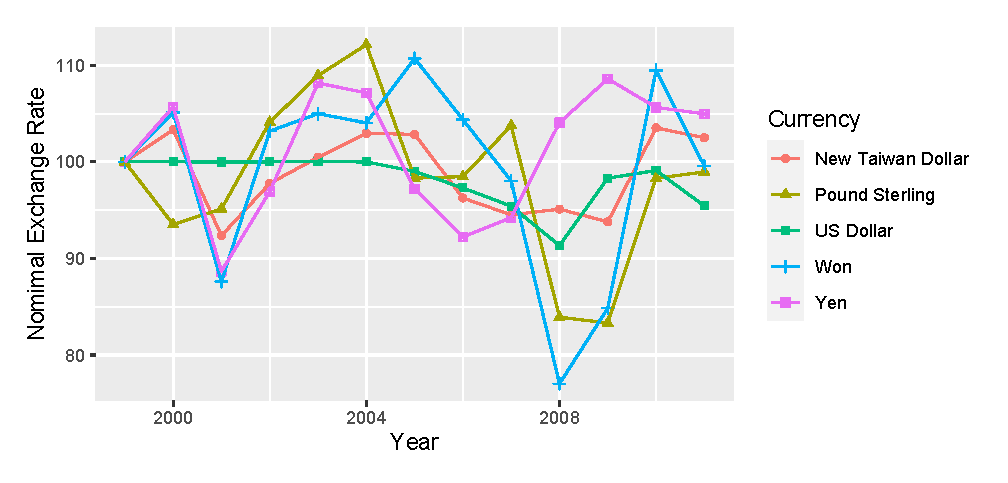
\includegraphics[width=1\textwidth]{figure/figure1.eps}
	\caption{Nominal exchange rates of China's major trading partners (1999-2011)}
	\label{fig3.1}
\end{figure}

\begin{figure}[htbp]
	\centering
	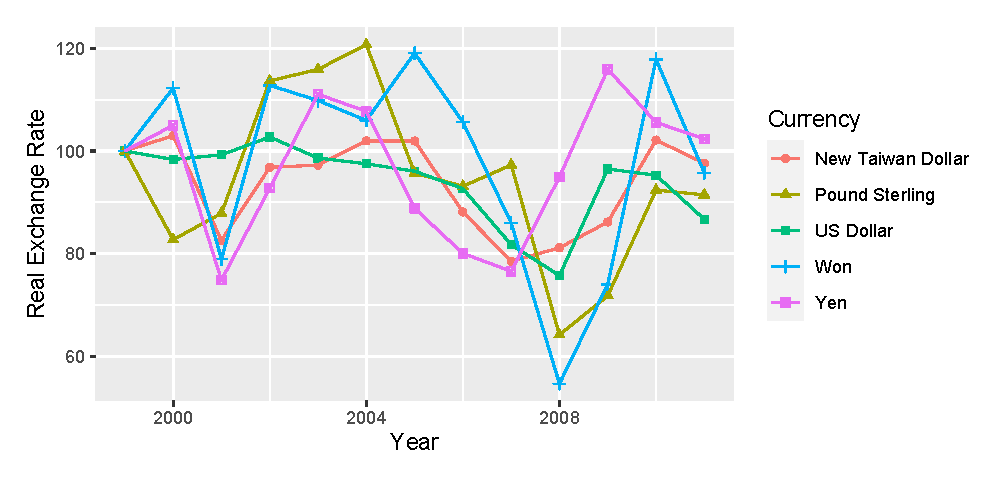
\includegraphics[width=1\textwidth]{figure/figure2.eps}
	\caption{Real exchange rates of China's major trading partners (1999-2011)}
	\label{fig3.2}
\end{figure}

In addition to nominal and real exchange rates, we also use the real GDP of the destination countries from PWT 10.0. The real GDP is computed with national-accounts growth rates. The controls of real GDP changes of the destination country, $\Delta RGDP_{ct}$, help us exclude the effect of economic growth on price movements. All macro variables including exchange rates and real GDPs are in annual terms to match the firm information survey.
\chapter{Empirical Framework}\label{sec-4.framework}
This section describes our econometric specifications and measurements of key variables of interest.

\section{Estimating Equations}

\subsection{Baseline estimations of exchange rate pass-through}

Since exchange rate pass-through is not an indicator that can be directly measured, we need to use panel data regression to estimate it. The first step goal is to estimate exchange rate pass-through as the elasticity of unit values changes to exchange rate changes using the firm-product-country details. Our strategy is based on the fixed effects regression. Specifically, we run a regression of import price changes on the bilateral real exchange rate changes between China and the source country, controlling the change of real GDP in the source country. The baseline equation refers to AIK\cite{aik2014} and LMX\cite{lmx2015} as below:

\begin{equation}
	\Delta \ln P^{D}_{i j c t}=\alpha+\beta^D \Delta \ln R E R_{c t}+\gamma \Delta \ln R G D P_{c t}+\xi_{i j c}+\tau_{t}+\varepsilon_{i j c t}
	\label{eq4.1}
\end{equation}

where $P_{ijct}$ represents the trade price of the product $i$ bought (sold) by firm $j$ from (to) country $c$ during year $t$.  $D \in$ \{Import, Export\} denotes the trade direction. Therefore, this equation could be used to estimate both import and export exchange rate pass-through with different values of D. $R E R_{c t}$ is the bilateral real exchange rate between Chinese RMB and currency in the country $c$. $RGDP_{ct}$ represents the real GDP of the source country deflated to the constant price level, which proxy for market demand. $\xi_{ijc}$ denotes the firm-product-country level fixed effects to capture any time-invariant unobserved factors for a combination of firm, product, and destination. These multi-dimensional fixed effects restrict unit value changes to price adjustments, rather than other changes in corporate trade decisions. $\tau_t$, the year dummies, control for macro-shocks that are common to all firms. We will alter the fixed effects setting in robustness checks.

To deal with possible non-stationarity of the panel, we use the first difference of the logarithms for prices $\Delta \ln P^{D}_{i j c t}$, real exchange rates $\Delta \ln R E R_{c t}$ and real GDP $\Delta \ln R G D P_{c t}$ to represent their annual rates of change. In this way, we transform the dynamic panel into a fixed effects regression. Therefore, using import price changes, the estimated coefficient of interest $\beta$ is the elasticity of price changes to exchange rate changes, i.e. import exchange rate pass-through. We also provide estimations for export exchange rate pass-through which is more common in past literature, where import prices are now replaced by export prices and the information of sources is replaced by which of destination markets. 

The real prices for export and import $P^{Import}_{i j c t}$ and $P^{Export}_{i j c t}$ are both denominated by the Chinese RMB in this paper. Using RMB as the denomination currency will make the coefficients on the import side and export side have different meanings. The level of coefficient $\beta^{D=Import}$ measures the completeness of import exchange rate pass-through, i.e. a higher $\beta$ means Chinese importers face more volatile import RMB prices during exchange rate shocks. However, for the export side,  $\beta^{D=Export}$ means the "incompleteness" of the export pass-through because a higher $\beta$ means Chinese exporters pass less exchange rate change to the destination market while having more volatile domestic currency prices. To be noticed, a majority of firms in our sample are both importers and exporters so they will appear in estimations of both exchange rate pass-through.

\subsection{Estimations with credit constraints}\label{seq-4.1.2}

Since our main focus is how firms' credit constraints affect exchange rate pass-through, we then include an interaction term of sectors’ financial vulnerability into the estimation function. Intuitively, firms operating in those financially vulnerable industries tend to have less access to enough funds to support their international trade activities, that is, they are subject to tighter credit constraints.

Therefore, we study the credit constraint effects on exchange rate pass-through across sectors with the following panel regression:

\begin{equation}
	\Delta \ln P^{D}_{ijct}=\alpha+\beta^D_{1} \Delta \ln RER_{ct}+\beta^D_{2} \Delta \ln RER_{ct} \cdot FV_{j}+\gamma \Delta \ln RGDP_{ct}+\xi_{ijc}+\tau_{t} +\varepsilon_{ijct}
	\label{eq4.2}
\end{equation}

where the variable $FV_{j}$ represents the financial vulnerability of the sector to which the firm $j$ belongs and the rest are the same as those in the baseline equation. The interaction coefficient $\beta_2$ represents the effect of credit constraints on exchange rate pass-through. A positive $\beta^{Import}_2$ for importers implies more credit-constrained importers have a more complete import exchange rate pass-through, while a positive $\beta^{Export}_2$ implies more credit-constrained exporters have a less complete exchange rate pass-through. The overall import ERPT for an importer $j$ is given by $\beta^D_{1} +\beta^{Import}_{2} FV_j$ and the export ERPT for an exporter $j$ is  $\beta^D_{1} +\beta^{Export}_{2} FV_j$.

Through this estimation strategy, we hope to scrutinize how the pricing behavior of Chinese importers in response to the exchange rate is affected by credit constraints and compare it with that of exporters. Although the functional forms for export and import pass-through are similar, the underlying mechanism could be different, which is one of our key innovation points. While credit-constrained exporters’ pricing decisions to deal with exchange rate shocks are mainly related to production and profit margin, the penetration effect of credit constraints on import prices is through a more direct channel, as the shortage of funds directly affects purchasing choices and bargaining.

\subsection{Estimations with additional factors}\label{sec-4.1.3}

After estimating exchange rate pass-through at the firm level and the impact of credit constraints on it, we need to go a step further to explore why. Through what channels will credit constraints affect the ability of importers to cope with exchange rate shocks? What other factors would exacerbate or diminish this effect? Are the effects of credit constraints fully explained by these controls?

In this part, we explore additional factors that affect firm-level import exchange rate pass-through. To do so, we introduce a vector $\mathbb{Z}_{jt}$ (or its lagged form $\mathbb{Z}_{jt-1}$) to include those additional factors and apply it to both control terms and interaction terms with real exchange rate changes: 

\begin{equation}
	\Delta \ln P^{D}_{ijct}=\alpha+[\beta^D_{1}+ \beta^D_{2} \cdot FV_{j}+\beta^D_{3} \cdot {\mathbb{Z}^{D}_{jt-1}}'] \Delta \ln RER_{ct} +\gamma \Delta \ln RGDP_{ct}+ {\mathbb{Z}^{D}_{jt}}' \eta+\xi_{ijc}+\tau_{t} +\varepsilon_{ijct}.
	\label{eq4.3}
\end{equation}

\begin{equation}
	\begin{aligned}
		\Delta \ln P^{D}_{ijct}=&\alpha+[\beta^D_{1}+ \beta^D_{2} \cdot FV_{j}+\beta^D_{3} \cdot {\mathbb{Z}^{D}_{jt-1}}'+\beta^D_{4} \cdot FV_{j} \cdot {\mathbb{Z}^{D}_{jt-1}}'] \Delta \ln RER_{ct} \\ &+\gamma \Delta \ln RGDP_{ct}+ {\mathbb{Z}^{D}_{jt}}' \eta+\xi_{ijc}+\tau_{t} +\varepsilon_{ijct}.
	\end{aligned}	
	\label{eq4.4}
\end{equation}

We will then use the estimation strategy of the form \ref{eq4.3} and \ref{eq4.4} to take into account various factors that may directly or indirectly affect exchange rate pass-through. We want to verify whether the effects of credit constraints are fully explained by some of these channels. Our firm-level data has the merit of containing information on its production, so we could connect the exchange rate pass-through with estimated firm-specific markup. We will also include trading partners later to measure the flexibility to choose alternative import sources. The coefficient of the interaction term between additional factors and real exchange rate movement $\beta_3$ represents the direct effects of those factors on the exchange rate pass-through other than through financial constraints. In equation \ref{eq4.4}, the triple interaction coefficient represents the indirect effects of those factors on the exchange rate pass-through through financial constraints. The same sign of $\beta_2$ and $\beta_4$ means that the factor enhances the effect of credit constraints, while the opposite sign means that it alleviates credit constraints.

Market share is another popular proxies for firm size or market power. For example, AIK (2014)\cite{aik2014} uses destination-specific market shares proxying for markup elasticity. When using market share as the additional factor, equation \ref{eq4.3} becomes the derivative form as below:

\begin{equation}
	\begin{aligned}
	\Delta \ln P^{D}_{ijct}=&\alpha+[\beta^D_{1}+ \beta^D_{2} \cdot FV_{j}+\beta^D_{3} \cdot S^{D}_{ijct}+\beta^D_4 \cdot {S^{D}_{ijct}}^2] \Delta \ln RER_{ct} \\
	&+\gamma \Delta \ln RGDP_{ct}+ \eta S^{D}_{ijct}+\xi_{ijc}+\tau_{t} +\varepsilon_{ijct}.
	\end{aligned}
	\label{eq4.5}
\end{equation}

The quadratic term for market share is used to test whether there is a non-monotonic relationship between exchange rate pass-through and market shares, such as the U-shape relationship documented by \cite{garetto2016} and \cite{devereux2017}. In addition to this, controlling for market share improves our estimation accuracy of the effect of credit constraints on exchange rate pass-through.

\section{Measurements}

\subsection{Unit value as trade price}

The customs records contain disaggregated trade values (denominated by US dollars) and quantities for each HS6 product $i$, each firm $j$, from (or to) each country $c$, in each year $t$, $V_{ijct}$, and $Q_{ijct}$. We first convert the value of the goods into RMB using the average exchange rate for the year. Then, the import and export prices we use are computed as unit values, defined as 

$$
P^{D}_{ijct}=\frac{V^{D}_{ijct}\cdot NER_{US,t}}{Q^{D}_{ijct}}
$$

where $D \in$ \{Import, Export\} and $NER_{US,t}$ is the annualized nominal exchange rate of US dollars in terms of RMB in year $t$. Because product categories are highly subdivided, we believe that the unit value is an ideal proxy for the transaction price.

Similar to real exchange rates, we take the first difference of the logarithm to represent price changes of a certain product across years. We will exclude observations with the annual growth rate of unit value in the top or bottom 1 percentile in the distribution, by HS2 product category and year, to avoid results being affected by extreme idiosyncratic factors other than some exchange rate adjustments.

\subsection{Credit constraints}\label{sec-4.2.2}

One of the most critical issues in our empirical strategy is to measure the extent of financial constraints. To deal with potential concurrent endogeneity, our measures of credit constraints are applied to each firm across the whole period. Following a widely recognized literature on the role of credit constraints in international trade (\cite{kroszner2007}; \cite{manova-wei-zhang2015}; \cite{fan-lai-li2015}), we use multiple financial vulnerability measures at the sector level to proxy for credit needs (demand for outside capital) and ability to resist financial risks. These measures are designed to reflect the nature of each industry which should be regarded as exogenous for each firm. If a firm is in a more financially vulnerable industry, it tends to face a tighter credit constraint, regardless of its operating conditions.

The first measure we use is external finance dependence ($ExtFin_j$), the share of capital expenditures not financed by operational cash flows. If external finance dependence is high, the industry is more financially vulnerable and firms in this industry are more credit constrained. The second measure is asset tangibility ($Tang_j$), which describes the share of the net value of tangible assets that firms can pledge as collateral to raise external finance, in its total book value. The third measure is the inventory-to-sales ratio ($Invent_j$), which measures the production cycle duration and the necessary working capital to maintain inventories and meet demand.  

To utilize the U.S. industry-level credit measures in the literature, we match the CIC industry code system used in China to the International Standard Industrial Classification (ISIC) system. We first convert the older ISIC Revision 2 3-digit and 4-digit industries from \cite{manova-wei-zhang2015} to match the newest ISIC Revision 3 codes; then we link the ISIC Revision 3 codes to the adjusted CIC codes in CIE datasets. Finally, we could match firms in the merged sample to those sector-level financial vulnerability measures. One-to-many situations may occur in the process of encoding matching. In this case, we construct the target variable for the new industry by averaging its source industries.

Although we construct three measures of credit constraints as in the literature, we will focus on the external finance dependence and tangibility in our later analysis. One important reason is that their interpretation can be linked to firms' exposure and resistance to financial frictions directly. In contrast, the inventory ratio may be connected to inventory management efficiency rather than liquidity and financial reasons. Following \cite{manova-wei-zhang2015}, we also construct the first principal component of external finance dependence and asset tangibility $FPC_j$, which increases with the former and falls with the latter. An industry with a higher $FPC_j$ is more financially sensitive if firms in it require more outside funds but own less collateralizable assets. Therefore, we could use $FPC_j$ as an aggregate measure to combine information about financial vulnerability from $ExtFin_j$ and $Tang_j$.

We have two major reasons why we use credit constraint measures based on US data in our main regressions. First, we want to remove the distortion by the limited credit supply in China and focus on the credit demand associated with sectoral characteristics. Second, the U.S. patterns of sectoral credit demand are proved persistent in a cross-country setting in the literature (\cite{kroszner2007}; \cite{manova-wei-zhang2015}; \cite{fan-lai-li2015}), especially when the industry classification is broadly defined. Intuitively, the financial needs of an industry may differ in level across countries, but the relative ranking between industries is supposed to be the same across countries, due to technical reasons specific to the industry itself.

Alternatively, we also compute credit needs based on Chinese firm-level information from CIE data. In addition to the already mentioned three measures, external finance dependence ($ExtFin_j$), asset tangibility ($Tang_j$), and inventory ratio ($Invent_j$), we include the fourth measure is R\&D intensity ($RD_j$), defined as the ratio of research and development expenditure to the total sales. Usually, R\&D activities are capital-intensive so it requires firms to pay a large fixed cost before production and sales. Therefore, firms in an R\&D-intensive industry should be more financially vulnerable. However, since we only have the information on firms' R\&D expenditure in and after 2005, which narrows the range of available samples, we will only use R\&D intensity as an auxiliary proxy variable. 

We adopt the measure of external finance dependence used by \cite{fan-lai-li2015}. Then we calculate the inventory ratio as the value of inventory over sales income, the asset tangibility as the value of fixed assets over total assets, and the R\&D intensity as R\&D spending over total sales income. To avoid credit constraints being endogenously affected by other corporate factors, we take the median of the firm-level credit constraint measure in the same CIC 2-digit industry as the industry-level credit constraint measure. Since the R\&D investment of a considerable number of companies is equal to 0, we choose to take the average rather than the median when calculating the R\&D intensity of the industry. The regression results using the Chinese industry measures are provided as robustness checks.

The summary statistics of the credit constraints measures in the firm-level data are shown in panels A and B in Table \ref{tab4.1}, respectively.

\begin{table}[htbp]
	\centering
	\caption{Summary Statistics of Credit Constrains Measures}
	\label{tab4.1}
	\resizebox{1.05\textwidth}{32mm}{
		\begin{threeparttable}
			\begin{tabular}{lcccccc}
				\toprule
				& \multicolumn{1}{l}{\#observations} & \multicolumn{1}{l}{Mean} & \multicolumn{1}{l}{Median} & \multicolumn{1}{l}{Std. dev} & \multicolumn{1}{l}{P10} & \multicolumn{1}{l}{P90} \\
				\textbf{Panel A: US Measures} &       &       &       &       &       &  \\
				$FPC_{j}$ &  1,745,511 & -7.12e-09 & -0.2706642 & 1 & -1.071394   & 1.072687 \\
				$ExtFin_{j}$ & 1,745,511 & -.0036698 & -0.05 & 0.3112002 & -0.25 & 0.28 \\
				$Tang_{j}$ & 1,745,511 & 0.3106788 & 0.32 & 0.0944181 & 0.1866667 & 0.43 \\
				$Invent_{j}$ & 1,745,511 & 0.1594069 & 0.1633333  & 0.0292352 & 0.115   & 0.1933333 \\
				\midrule
				& \multicolumn{1}{l}{\#observations} & \multicolumn{1}{l}{Mean} & \multicolumn{1}{l}{Median} & \multicolumn{1}{l}{Std. dev} & \multicolumn{1}{l}{P10} & \multicolumn{1}{l}{P90} \\
				\textbf{Panel B: Chinese Measures} &       &       &       &       &       &  \\
				$ExtFin_{j}$ & 1,745,511 & -0.6479498 & -0.47 & 0.6746751 & -1.32 & -0.1  \\
				$Tang_{j}$ & 1,745,511 & 0.3332769 & 0.3268749 & 0.0648019 & 0.2390799 & 0.4317028 \\
				$Invent_{j}$ & 1,745,511 & 0.1102537 & 0.1030875  & 0.0274747 & 0.0778921   & 0.1348336 \\
				$R\&D_{j}$ & 1,745,511 & 0.0168278 & 0.012111 & 0.0142106 & 0.0053125  & 0.0281532 \\
				\bottomrule
			\end{tabular}
			\begin{tablenotes}
				\footnotesize
				\item[*] This table shows the summary statistics of credit constraint measures. Panel A describes the measures calculated using US data while panel B shows the alternative Chinese version. All variables are unitless, the numerical size only means relative rank.
			\end{tablenotes}
		\end{threeparttable}
	}
\end{table}

\subsection{Import sources and export markets}\label{sec-4.2.3}
Following the literature about import sourcing, an importer's sourcing diversity could increase its bargaining power in import prices in addition to its production characteristics. We want to test how importers' sourcing diversity affects exchange rate pass-through. We provide a simple measure for the firm-product level sourcing diversity $Source_{ijt}$ as the number of source countries from which an importer $j$ imports a certain HS6 product type $i$ in year $t$. 

Similarly, for exporters, we count the number of destination countries to which an exporter exports a certain HS6 product type $i$ as the firm-product-level selling measure, $Market_{ijt}$. Controlling other variables, the number of export markets for the same product can measure its export network diversity. In a robustness test, we use the firm-year fixed effect to control for differences in import and export diversity caused by firm size.

\subsection{Firm-level markup}\label{sec-4.2.4}

In the discussion, we argue that credit constraints will affect the "absorptive capacity" of exchange rate shocks other than the firm's attributes in sales. In the following work, we will control markup to test the conjectures concretely. Referring to \cite{bkl2021}, even without direct measures of prices and marginal cost, we can still estimate the firm-level markup, using the structural assumptions of \cite{dlw2012} (DLW hereafter) and GMM estimation method.

Simply put, DLW (2012)\cite{dlw2012} derives the firm-specific markup as the ratio of an input factor's output elasticity to its firm-specific factor payment share $\mu_{t}=\theta_{t}^{X}\left(\alpha_{t}^{X}\right)^{-1}$, where $\alpha_{t}^{X}$ is the share of expenditures on input X in total sales and $\theta^X_t$ denotes the output elasticity on an input X. The major difficulty is calculating the firm-specific output elasticity concerning materials, which requires estimating firm-specific production functions. We apply the methodology of \cite{acf2015} to address the endogeneity of inputs, assuming a 3rd-order translog gross output production function in capital, labor, and material inputs:

$$
\begin{aligned}
y_{t}= &\beta_{k} k_{t}+\beta_{l} l_{t}+\beta_{i} m_{t}+\beta_{k 2} k_{t}^{2}+\beta_{l 2} l_{t}^{2}+\beta_{m 2} m_{t}^{2}+\beta_{k l} k_{ t} l_{t}+\beta_{k m} k_{t} m_{t}+\beta_{l m} l_{t} m_{t}+\beta_{k 3} k_{t}^{3}\\
&+\cdots+\omega_{t}+\epsilon_{t}.
\end{aligned}
$$

In practice, we need to construct four production variables in log form: real output value $y_t$, persons engaged $l_t$, real fixed assets at current value $k_t$, and real material inputs $m_t$. Real output values are deflated by output deflators, while real fixed assets and real material inputs are deflated by investment deflators and input deflators, respectively. The deflators are constructed as in \cite{brandt2012}.

\subsection{Market share}\label{sec-4.2.5}

In addition to the extensive diversity measured by the number of import sources or export markets, we also use a firm's share in a specific import or export market to describe its intensive competitiveness.

Following AIK\cite{aik2014} and \cite{devereux2017}, we define import market share as a firm’s value share in the import market, within a given HS6 product category. Therefore, a single firm can have multiple import market shares for multiple products. Our definition of import market share is also year specific, and so a firm’s import market share can vary over time. 

$$
S^{D}_{ijct} \equiv \frac{v^{D}_{ijct}}{\sum_{j^{\prime} \in J_{ict}} v^{D}_{ij^{\prime}ct}}
$$

where $D \in$ \{Import, Export\}. The capital letter $J$ denotes the set of potential competitors in the same product-specific market. 

The destination-specific export market share proxy is similarly defined as the value share of a firm relative to all Chinese exporters in our sample who export the same product to the same market. Since we only have data from China Customs, our export market share $S^{D}_{ijct}$ is relative to other Chinese firms. The external competitive stance in a particular sector-destination pair is also common for all Chinese exporters in that country and hence our measure captures all relevant variation in market share between firms in our sample.
\chapter{Empirical Results}\label{sec-5.results}
In this section, we will present our major empirical results using the samples and strategies described above. First, we show the estimated import exchange rate pass-through is rather incomplete while the export exchange rate pass-through is very close to complete. Second, we show that both importers and exporters with tighter credit constraints have more complete pass-through. Finally, we present the results with firm heterogeneity to explore factors affecting importers' capacity to absorb exchange rate and the role of credit constraints among them.

\section{Import Pass-through vs Export Pass-through}\label{sec-5.1}

Past literature on firm-level evidence of exchange rate pass-through mainly focuses on exporters' price-setting behaviors. Importers are likely to be more than simple price takers, which gives us a new perspective on exchange rate pass-through. Now we take a closer look at how real exchange rate fluctuations affect import prices and export prices differently in China. The results for import exchange rate pass-through versus export exchange rate pass-through are shown in table \ref{tab5.1} using different samples.

\begin{table}[htbp]
	\centering
	\caption{Baseline Estimations of Exchange Rate Pass-Through}
	\begin{threeparttable}
	\begin{tabular}{lcccc}
		\toprule
		& (1)   & (2)   & (3)   & (4) \\
		\midrule
		Panel A & \multicolumn{4}{c}{Import} \\
		& Whole & Matched & Top 50 & Top 20 \\
		\midrule
		$\Delta \ln RER_{ct}$ & 0.179*** & 0.357*** & 0.354*** & 0.344*** \\
		& (0.003) & (0.015) & (0.015) & (0.016) \\
		$\Delta \ln RGDR_{ct}$ & -0.133*** & 0.263*** & 0.282*** & 0.333*** \\
		& (0.026) & (0.090) & (0.091) & (0.097) \\
		Year FE  & Yes   & Yes   & Yes   & Yes \\
		Firm-product-country FE & Yes   & Yes   & Yes   & Yes \\
		Observations & 8409682 & 1792020 & 1781948 & 1684798 \\
		\midrule
		Panel B & \multicolumn{4}{c}{Export} \\
		& Whole & Matched & Top 50 & Top 20 \\
		\midrule
		$\Delta \ln RER_{ct}$ & 0.050*** & 0.031*** & 0.039*** & 0.065*** \\
		& (0.002) & (0.005) & (0.006) & (0.009) \\
		$\Delta \ln RGDR_{ct}$ & -0.102*** & -0.083** & -0.118*** & -0.082 \\
		& (0.010) & (0.037) & (0.042) & (0.056) \\
		Year FE  & Yes   & Yes   & Yes   & Yes \\
		Firm-product-country FE & Yes   & Yes   & Yes   & Yes \\
		Observations & 11173463 & 1793974 & 1611410 & 1251147 \\
		\bottomrule
	\end{tabular}
	\begin{tablenotes}
		\footnotesize
		\item[*] Standard errors in parentheses; *, **, and *** indicate significance at 10\%, 5\% and 1\% levels. Panel A shows the estimations for import ERPT while panel B shows the export ERPT. The dependent variable is the price change $\Delta \ln P_{ijct}$. Column (1) uses the long sample from 2000 to 2011. Column (2) uses the matched sample from 2000 to 2007. Columns (3) and (4) use finer sub-samples with only top 50 and top 20 partners ranked by total trade value. All regressions include firm-product-country fixed effects and year fixed effects. 
	\end{tablenotes}
	\end{threeparttable}
	\label{tab5.1}
\end{table}

We report the baseline estimates of import exchange rate pass-through in panel A. Column (1) shows the import exchange rate pass-through using equation (1) for the long sample from 2000 to 2011, including all companies that appear at least once in customs records, whether or not they are registered in the CIE database. Column (2) shows the results for import exchange rate pass-through for the matched sample (importers registered in the CIE database from 2000 to 2007). The pass-through coefficient in column (2) is larger than the one in column (1), yet both are incomplete. The average import exchange rate pass-through for China in the long sample is around 18\%, while in the matched sample about 39\%. The latter ERPT means that the import prices denominated in RMB will increase by about 3.9\% during a 10\% real depreciation and decrease by the same amount during a 10\% appreciation. Column (3) and column (4) report the import pass-through among a subset of the matched sample including only the top 50 and top 20 trading partners by import value. The results in those subsamples of top partners are slightly less complete than those in column (2), yet the levels are of similar magnitude. Import price fluctuations will reflect nearly one-third of exchange rate fluctuations, with the remainder absorbed by foreign currency price fluctuations. These results imply that Chinese importers have to bear less than half but still considerable cost fluctuations due to exchange rate shocks. 

Accordingly, estimates of export exchange rate pass-through are recorded in panel B. Similar to which in panel A for imports, column (1) and column (2) in panel B show the export exchange pass-through using the long sample and the matched sample. Column (3) and column (4), in turn, show the export price pass-through to major export destinations. The estimated export pass-through in each column equals one minus the coefficient at the row of $\Delta lnRER_{ct}$. The export pass-through ranges from 93.3\% for the top 20 countries to 96.6\% for the matched sample, which is near complete. The strikingly almost complete ERPT into RMB export price echoes the finding of LMX\cite{lmx2015}. Specifically, 95\% export ERPT means that a 10\% real appreciation of RMB concerning a destination market is associated with a 0.5\% decrease in the RMB price while a 9.5\% increase in foreign currency price. RMB price adjusts very little with exchange rate fluctuations. Interestingly, this price increase may be particularly pronounced in Sino-US trade, as the yuan has steadily appreciated against the dollar from 2000 to 2007. Most Chinese exporters have no choice but to pass all exchange rate swings to their destination prices, regardless of potential better monopolistic competition strategies.

From the comparison, it can be seen that the exchange rate-price pass-through in China's import side is much lower than that in the export side. That is to say, for Chinese firms, when RMB depreciates against the currencies of major trading partners, export prices denominated in RMB will not rise significantly, but their import costs will rise sharply; on the contrary; when the real exchange rate of RMB appreciates, export prices in RMB will decrease only to a limited extent, and their import costs will increase dramatically drop. If we consider a typical two-way trader in China who simultaneously imports and exports from two groups of countries with strong correlations in exchange rate fluctuations, a devaluation of the local currency will reduce his unit profits, while an appreciation of the local currency will widen his profit margins. We call this phenomenon the asymmetry of the import and export exchange rate pass-through, which exposes Chinese trading companies to two-way exchange rate risks.

\section{Effects of Credit Constraints}\label{sec-5.2}

Another goal of our paper is to assess how importers with varying degrees of financial vulnerability absorb exchange rate fluctuations when the home currency depreciates or appreciates. We evaluate the consequences of credit constraints on the firms' price responses to exchange rate shocks using equation \ref{eq4.2} in section \ref{seq-4.1.2}. Table \ref{tab5.2} presents differences in exchange rate pass-through into import prices and export resulting from the industry-level credit demand heterogeneity. Panel A reports the results for credit constraints and import pass-through and panel B reports the comparing results for the export side. 

\begin{table}[htbp]
	\centering
	\caption{Effects of Credit Constraints on Exchange Rate Pass-Through}
	\begin{threeparttable}	
	\begin{tabular}{lcccc}
		\toprule
		& (1)   & (2)   & (3)   & (4) \\
		\midrule
		Panel A & \multicolumn{4}{c}{Import} \\
		& FPC   & External Finance & Tangibility & Inventory \\
		\midrule
		$\Delta \ln RER_{ct}$ & 0.123*** & 0.218*** & 1.175*** & -0.739*** \\
		& (0.016) & (0.016) & (0.033) & (0.069) \\
		$\Delta \ln RGDR_{ct}$ & 0.314*** & 0.323*** & 0.283*** & 0.273*** \\
		& (0.090) & (0.090) & (0.090) & (0.090) \\
		$\Delta \ln RER_{ct}*FPC_{j}$ & 0.379*** &       &       &  \\
		& (0.010) &       &       &  \\
		$\Delta \ln RER_{ct}*ExtFin_{j}$ &       & 1.159*** &       &  \\
		&       & (0.029) &       &  \\
		$\Delta \ln RER_{ct}*Tang_{j}$ &       &       & -3.305*** &  \\
		&       &       & (0.117) &  \\
		$\Delta \ln RER_{ct}*Invent_{j}$ &       &       &       & 6.305*** \\
		&       &       &       & (0.389) \\
		Year FE  & Yes   & Yes   & Yes   & Yes \\
		Firm-product-country FE & Yes   & Yes   & Yes   & Yes \\
		Observations & 1792020 & 1792020 & 1792020 & 1792020 \\
		\midrule
		Panel B & \multicolumn{4}{c}{Export} \\
		& FPC   & External Finance & Tangibility & Inventory \\
		\midrule
		$\Delta \ln RER_{ct}$ & 0.039*** & 0.034*** & -0.030** & 0.102*** \\
		& (0.006) & (0.005) & (0.015) & (0.030) \\
		$\Delta \ln RGDR_{ct}$ & -0.084** & -0.083** & -0.084** & -0.083** \\
		& (0.037) & (0.037) & (0.037) & (0.037) \\
		$\Delta \ln RER_{ct}*FPC_{j}$ & -0.019*** &       &       &  \\
		& (0.004) &       &       &  \\
		$\Delta \ln RER_{ct}*ExtFin_{j}$ &       & -0.045*** &       &  \\
		&       & (0.013) &       &  \\
		$\Delta \ln RER_{ct}*Tang_{j}$ &       &       & 0.230*** &  \\
		&       &       & (0.053) &  \\
		$\Delta \ln RER_{ct}*Invent_{j}$ &       &       &       & -0.412** \\
		&       &       &       & (0.171) \\
		Year FE  & Yes   & Yes   & Yes   & Yes \\
		Firm-product-country FE & Yes   & Yes   & Yes   & Yes \\
		Observations & 1793974 & 1793974 & 1793974 & 1793974 \\
		\bottomrule
	\end{tabular}
	\label{tab5.2}
	\begin{tablenotes}
		\footnotesize
		\item[*] Standard errors in parentheses; *, **, and *** indicate significance at 10\%, 5\% and 1\% levels. The dependent variable is the price change $\Delta \ln P_{ijct}$. Columns (1)-(4) use different measures of credit constraints calculated using U.S. data. Panel A shows the effects of credit constraints on import ERPT while panel B shows their effects on export ERPT. All regressions include firm-product-country fixed effects and year fixed effects.
	\end{tablenotes}
	\end{threeparttable}
\end{table}

We are particularly interested in the coefficients of the interaction terms. Note that a larger elasticity coefficient on the import side implies more complete exchange rate-price pass-through, and similarly a positive cross-term coefficient implies that the magnitude of this variable is positively related to exchange rate pass-through. Using the first principal component of external finance dependence and asset tangibility $FPC_j$ to measure financial vulnerability $FV_j$, we see that import exchange rate pass-through is more complete in financially more vulnerable sectors, relative to financially less vulnerable sectors (column 1, row 3). Columns (2) and (3) separately show the effects of external finance dependence and asset tangibility on importers' exchange rate pass-through. Consistent with the definition that higher external finance dependence implies tighter credit constraints faced by firms while higher asset tangibility can alleviate them, we observe a positive coefficient for the former (row 5) and a negative coefficient for the latter (row 6). When we use the auxiliary measure $Invent_j$, we further observe that the effect on exchange rate pass-through is positive (column 4). Overall, the coefficient $\beta^{Import}_2$ of the interaction term $\Delta \ln RER_{ct} \cdot FV_{j}$ is positive and significant at the 1\% level. Our evidence supports the intuition that exchange rate fluctuations are more likely to be reflected in unstable import costs for importers in more financially vulnerable industries because they have weak bargaining power in the international market. External financing dependence, internal collateral capacity, and inventory turnover all act jointly and separately on the exchange rate pass-through of importers.

By substituting the superscript D in equation \ref{eq4.2} to export, we obtain a comparative result of the effect of credit constraints on export price pass-through. Estimates in columns (1), (2), and (4) all show significantly negative coefficients on interaction terms while column (3) shows a negative significant coefficient. The estimates suggest that financial constraints lead export exchange rate pass-through to a more complete degree, although the original result is already close to complete. These results verified the conclusion of \cite{strasser2013} who argues that financially constrained firms have higher export price pass-through compared to unconstrained firms. That is to say, credit constraints restrict exporters from absorbing exchange rate shocks, potentially because firms need external finance to apply pricing-to-market strategies in foreign markets.

Comparing panel A and panel B, although the import ERPT is still much lower than export ERPT, we can reach a consistent conclusion that credit constraints steer both of them toward a more complete direction. Following the analysis in section \ref{sec-5.1}, credit constraints expose Chinese manufacturing firms to greater exchange rate risk in international trade. Exporters with more vulnerable credit are forced to sharply lower destination prices when RMB depreciate compared to those with unrestricted credit, while RMB income remained relatively unchanged, and importers’ costs rose more significantly; in contrast, when RMB appreciates, restricted exporters will increase destination prices more, even if it means losing their competitive advantages, and importers' costs will be reduced at this time. For credit-constrained two-way traders, given import sources and export markets cannot be adjusted quickly, the unit profit margin is more sensitive to exchange rate fluctuations.

Nonetheless, the direction in which credit constraints affect the exchange rate pass-through on the export side and the import side is the same, the underlying channels may work differently. Following \cite{strasser2013}, a higher external finance premium causes higher marginal costs. Thus, firms with binding financial constraints have no choice but set higher prices and face a higher price elasticity of demand. When there is an exchange rate shock, the optimal choice is to adjust their markups but credit-constrained firms can do so only to a limited extent because they have narrower profit margins. However, for import ERPT, credit constraints can directly affect how buyers pay. Adequate credit or cash reserves give importers a better bargaining chip, for example, by allowing them to negotiate longer-term purchase agreements, where exchange rate fluctuations will be more borne by international sellers. In contrast, a credit-strapped importer may not have the buffers to transfer risk, so it must accept current exchange rate settlements, although that means taking on more volatile prices.

\section{Sourcing Diversity and Credit Constraints}

In this section, we further study the factors that directly affect the purchasing side. As emerged in an intuitive guess, a potential mechanism through which financial constraints affect an importer's bargaining power with foreign suppliers is its outside sourcing options. Companies with more trading partners can flexibly adjust the weight of imports from different countries. Firms with heterogeneous sourcing capacity may thus be affected by credit constraints by different extent. 

Therefore, we employ equation \ref{eq4.4} to include the number of import sources described in section \ref{sec-4.2.3}. The estimation results are reported in the below table \ref{tab5.3} and confirm the empirical relevance of differences in sourcing diversity across firms. Similarly, results for sales destination diversity on the export side are provided in panel B \ref{tabA.1} as a comparison.

\begin{table}[htbp]
	\centering
	\caption{Import Sources and Effects of Credit Constraints on Import Exchange Rate Pass-Through}
	\begin{threeparttable}
	\begin{tabular}{lcccc}
		\toprule
		& (1)   & (2)   & (3)   & (4)    \\
		\midrule
		Panel A & \multicolumn{4}{c}{Import} \\
		 & \#Sources & \#Sources+ & \#Sources+ & \#Sources+	 \\
		&       & FPC &External & Tangibility \\
		&       & &Finance &			\\
		\midrule
		$\Delta \ln RER_{ct}$ & 0.433*** & 0.177*** & 0.274*** & 1.386*** \\
		& (0.017) & (0.019) & (0.018) & (0.040) \\
		$\Delta \ln RGDR_{ct}$ & 0.250*** & 0.292*** & 0.297*** & 0.267*** \\
		& (0.090) & (0.090) & (0.090) & (0.090) \\
		$\#Source_{ijt}$ & -0.021*** & -0.016*** & -0.016*** & -0.050*** \\
		& (0.002) & (0.003) & (0.003) & (0.006) \\
		$\Delta \ln RER_{ct}*FPC_{j}*\#Source_{ijt}$ &       & -0.014*** &       &  \\
		&       & (0.002) &       &  \\
		$\Delta \ln RER_{ct}*FPC_{j}$ &       & 0.443*** &       &  \\
		&       & (0.012) &       &  \\
		$\Delta \ln RER_{ct}*ExtFin_{j}*\#Source_{ijt}$ &       &       & -0.054*** &  \\
		&       &       & (0.006) &  \\
		$\Delta \ln RER_{ct}*ExtFin_{j}$ &       &       & 1.410*** &  \\
		&       &       & (0.037) &  \\
		$\Delta \ln RER_{ct}*Tang_{j}*\#Source_{ijt}$ &       &       &       & 0.104*** \\
		&       &       &       & (0.026) \\
		$\Delta \ln RER_{ct}*Tang_{j}$ &       &       &       & -3.790*** \\
		&       &       &       & (0.148) \\
		Year FE  & Yes   & Yes   & Yes   & Yes \\
		Firm-product-country FE & Yes   & Yes   & Yes   & Yes \\
		Observations & 1792020 & 1792020 & 1792020 & 1792020 \\
		\bottomrule
	\end{tabular}
	\begin{tablenotes}
	\footnotesize
	\item[*] Standard errors in parentheses; *, **, and *** indicate significance at 10\%, 5\% and 1\% levels. The dependent variable is the price change $\Delta \ln P_{ijct}$. Columns (2)-(4) use different measures of credit constraints calculated using U.S. data. Panel A shows the effects of credit constraints on import ERPT while panel B shows their effects on export ERPT. Panel B is shown in Appendix \ref{tabA.1}. All regressions include firm-product-country fixed effects and year fixed effects.
	\end{tablenotes}
	\end{threeparttable}
	\label{tab5.3}
\end{table}

The estimates for intersection terms between import sources and real exchange rate changes are displayed in column (1). We find that importers who import a certain product from more sources will have a less complete pass-through. This is consistent with our hypothesis that importers with more alternative sourcing options will have less complete pass-through. Interestingly, exporters who export to more destinations (both for a certain product or in total) will have a slightly more complete pass-through. In other words, the diversity of import sources for the same product can significantly enhance the stability of import prices, but the diversity of export markets does not.

In columns (2)-(4), after adding interactions, we find the effects of credit constraints still exist while the triple interaction terms with the number of sources have the opposite and significant coefficients. That means a wider sourcing base will mitigate the effects of credit constraints, in addition to its own effect on pass-through. We continue to observe that this triple interaction effect only works for the import side in panel A but not for the export side in panel B (attached in appendix \ref{tabA.1}). The opposing effects of credit constraints and purchasing diversity on exchange rate pass-through confirm our conjecture about the bargaining power of importers. If a firm can import the same product from more sources, it has more flexibility in the face of bilateral exchange rate shocks in individual markets. In other words, the constrained firms with more import sources have more ways to escape the unfavorable exchange rate risk. A more diverse importer can either switch from one source to another to reduce costs (trade diversion effect), or make a more credible threat to negotiate a more stable price. 
\chapter{More Discussions}\label{sec-6.discussion}

\section{Firm Heterogeneity in Markup}

Given that credit constraints play an important role in China's import exchange rate pass-through, we proceed to analyze how different factors participate in determining import exchange rate pass-through, and whether they can replace credit constraints or not. One major argument in the literature is that firms with different sales markup may have heterogeneous responses to exchange rate shocks as suggested by \cite{bmm2012} and \cite{lmx2015}. The same logic could also apply to import exchange rate pass-through. Besides, \cite{llz2018} provide microeconomic evidence that both internal finance and external credit supply significantly promote firms' sales growth rates. Following the empirical framework in section \ref{sec-4.1.3}, we add estimated firm-level markup into interactions, and the results are shown in below table \ref{tab6.1}.

\begin{table}[htbp]
	\centering
	\caption{Heterogeneous Markup and Effects of Credit Constraints on Import Exchange Rate Pass-through}
	\begin{threeparttable}
		\begin{tabular}{lcccc}
			\midrule          & (1)   & (2)   & (3)   & (4)     \\
			\midrule
			Panel A & \multicolumn{4}{c}{Import} \\
			& Markup & Markup+& Markup+ & Markup+      \\
			&       &FPC& External & Tangibility        \\
			&       & & Finance &  	          \\
			\midrule
			$\Delta \ln RER_{ct}$ & 0.459*** & 0.310*** & 0.431*** & 1.419***   \\
			& (0.045) & (0.045) & (0.045) & (0.058) \\
			$\Delta \ln RGDP_{ct}$ & 0.329*** & 0.376*** & 0.389*** & 0.343*** \\
			& (0.106) & (0.106) & (0.106) & (0.106)  \\
			$\Delta \ln RER_{ct}$*$Markup_{jt-1}$ & -0.073** & -0.157*** & -0.163*** & -0.112*** \\
			& (0.030) & (0.030) & (0.031) & (0.030) \\
			$\Delta \ln RER_{ct}$*$FPC_{j}$ &       & 0.414*** &       &  \\
			&       & (0.011) &       &   \\
			$\Delta \ln RER_{ct}$*$ExtFin_{j}$ &       &       & 1.232*** &  \\
			&       &       & (0.034) &   \\
			$\Delta \ln RER_{ct}$*$Tang_{j}$  &       &       &       & -3.692*** \\
			&       &       &       & (0.139) \\
			$Markup_{jt-1}$ & 0.013** & 0.009 & 0.007 & 0.012**  \\
			& (0.006) & (0.006) & (0.006) & (0.006)  \\
			Year FE  & Yes   & Yes   & Yes   & Yes       \\
			Firm-product-country FE & Yes   & Yes   & Yes   & Yes       \\
			Observations & 1411106 & 1411106 & 1411106 & 1411106  \\
			\bottomrule
		\end{tabular}
		\begin{tablenotes}
			\footnotesize
			\item[*] Standard errors in parentheses; *, **, and *** indicate significance at 10\%, 5\% and 1\%. The dependent variable is the price change $\Delta \ln P_{ijct}$. Columns (2)-(4) use different measures of credit constraints calculated using U.S. data. Panel A shows the effects of markup and credit constraints on import ERPT while panel B shows their effects on export ERPT. Panel B is shown in Appendix \ref{tabA.2}. All regressions include firm-product-country fixed effects and year fixed effects.
		\end{tablenotes}
	\end{threeparttable}
	\label{tab6.1}
\end{table}

Panel A shows how markup affects import ERPT in addition to credit constraints and panel B (attached in \ref{tabA.2}) shows the comparison results for export ERPT. Column (1) shows the direct effects of firm-level markup on exchange rate pass-through. Columns (2) to (4) add the first principal component, external finance dependence and asset tangibility to the regression respectively. All columns control for the lag term of markup.

From the coefficients of interaction terms in panel A, firms with higher markup have lower degrees of import pass-through while firms. The effects of financial constraints are still significant and robust as in section \ref{sec-5.2} after controlling for markup. The coefficients in panel B \ref{tabA.2} imply a similar conclusion. Exporters with higher markup have lower export pass-through. In other words, higher markup on the exchange rate pass-through work in the opposite direction with tighter credit constraints. However, the coefficients in rows (4)-(6) are significant respectively, indicating that markup cannot fully explain the effect of credit constraints, which is consistent with \cite{xu-guo2021}.

The explanation for import price absorptive capacity seems more complicated than which for export ERPT. BMM\cite{bmm2012} documents that more productive firms react to depreciation (or appreciation) by adjusting more markup and less export volume, keeping local market prices relatively stable, which means a less complete pass-through. This explanation hinges on endogenous markup over marginal costs where less elastic demand allows them to adjust markups more extensively during currency fluctuations. However, at the import side, there are other factors that influence the sourcing capacity upon exchange rate movements. In any case, the effects of credit constraints are not offset or replaced by the sales factors, so the conclusions in section \ref{sec-5.2} about credit constraints remain valid.

\section{Firm Heterogeneity in Market Share}

In this section, we first provide the regression results of equation \ref{eq4.5} with the market share and its square term constructed in section \ref{sec-4.2.5}. The results are presented in Table \ref{tab6.2}. The coefficient estimates for $\beta_3$ and $\beta_4$ can be used to map out the ERPT–import market share relationship.

\begin{table}[htbp]
	\centering
	\caption{Market Share and Effects of Credit Constraints on Import Exchange Rate Pass-through}
	\begin{threeparttable}
		\begin{tabular}{lccccc}
			\toprule
			& (1)   & (2)   & (3)   & (4) & (5)\\
			\midrule
			Panel A & \multicolumn{5}{c}{Import} \\
			& MS    & $MS^2$ & FPC   & External & Tangibility \\
			&       &       &       & Finance &  \\
			\midrule
			$\Delta \ln RER_{ct}$ & 0.392*** & 0.381*** & 0.119*** & 0.220*** & 1.175*** \\
			& (0.016) & (0.016) & (0.018) & (0.017) & (0.033) \\
			$\Delta \ln RGDP_{ct}$ & 0.247*** & 0.251*** & 0.314*** & 0.321*** & 0.280*** \\
			& (0.090) & (0.090) & (0.090) & (0.090) & (0.090) \\
			$\Delta \ln RGDP_{ct}*MS_{ijct}$ & -0.305*** & 0.155 & 0.677*** & 0.556*** & 0.546*** \\
			& (0.042) & (0.156) & (0.156) & (0.156) & (0.156) \\
			$\Delta \ln RGDP_{ct}*MS^2_{ijct}$ &       & -0.531*** & -0.941*** & -0.837*** & -0.846*** \\
			&       & (0.173) & (0.173) & (0.173) & (0.173) \\
			$\Delta \ln RER_{ct}$*$FPC_{j}$ &       &       & 0.379*** &       &  \\
			&       &       & (0.010) &       &  \\
			$\Delta \ln RER_{ct}$*$ExtFin_{j}$ &       &       &       & 1.156*** &  \\
			&       &       &       & (0.029) &  \\
			$\Delta \ln RER_{ct}$*$Tang_{j}$ &       &       &       &       & -3.290*** \\
			&       &       &       &       & (0.118) \\
			$MS_{ijpt}$    & -0.012 & -0.009 & -0.002 & -0.004 & -0.003 \\
			& (0.012) & (0.012) & (0.012) & (0.012) & (0.012) \\
			Year FE  & Yes   & Yes   & Yes   & Yes   & Yes \\
			Firm-product-country FE & Yes   & Yes   & Yes   & Yes   & Yes \\
			Observations & 1792020 & 1792020 & 1792020 & 1792020 & 1792020 \\
			\bottomrule
		\end{tabular}
		\begin{tablenotes}
			\footnotesize
			\item[*] Standard errors in parentheses; *, **, and *** indicate significance at 10\%, 5\% and 1\%. The dependent variable is the price change $\Delta \ln P_{ijct}$. Columns (3)-(5) use different measures of credit constraints calculated using U.S. data. Panel A shows the effects of market share and credit constraints on import ERPT while panel B shows their effects on export ERPT. Panel B is shown in Appendix \ref{tabA.3}. All regressions include firm-product-country fixed effects and year fixed effects.
		\end{tablenotes}
	\end{threeparttable}
	\label{tab6.2}
\end{table}

In columns (1) and (2), we add the primary and quadratic terms of market share to the baseline estimation of ERPT in turn. In columns (3)-(4), we further include the effects of external finance dependence and asset tangibility on top of which in column (2). Panel B shows the results for export side. We find that there is evidence of a negative relationship between import pass-through and market share; however, the coefficient for the linear interaction term is positive, while the strong negative effect lies on the squared interaction term, suggesting some curvature in this relationship. The effect of market share on export ERPT is not significant. 

In addition, we also perform group regressions by market share quartile and report the results in table \ref{tab6.2}. Columns (1)-(4) show the import exchange rate pass-through for importers within each quartile of the market share distribution (0-25\%, 25\%-50\%, 50\%-75\%, 75\%-100\%), respectively. Panel B in turn shows the results for exporters within different quartiles in the market share distribution. Results for each quartile group with interaction terms of credit constraints are not provided here but are available upon request. Roughly speaking, the import exchange rate pass-through and market share show a hump-shaped (inverted U-shaped) relationship, and the export exchange rate pass-through coefficient (weakly) decreases with the market share (towards complete price pass-through in upper quartiles).

\begin{table}[htbp]
	\centering
	\caption{Estimations of Exchange Rate Pass-Through by Market Share Quartile}
	\begin{threeparttable}
		\begin{tabular}{lcccc}
			\toprule
			& (1)   & (2)   & (3)   & (4) \\
			\midrule
			Panel A & \multicolumn{4}{c}{Import} \\
			& 1st   & 2nd   & 3rd   & 4th \\
			\midrule
			$\Delta \ln RER_{ct}$ & 0.222*** & 0.378*** & 0.404*** & 0.242*** \\
			& (0.056) & (0.042) & (0.032) & (0.020) \\
			$\Delta \ln RGDP_{ct}$ & -0.371 & 0.444* & 0.314* & -0.054 \\
			& (0.324) & (0.241) & (0.179) & (0.129) \\
			Year FE  & Yes   & Yes   & Yes   & Yes \\
			Firm-product-country FE & Yes   & Yes   & Yes   & Yes \\
			Observations & 372447 & 450728 & 492016 & 476829 \\
			\midrule
			Panel B & \multicolumn{4}{c}{Export} \\
			& 1st   & 2nd   & 3rd   & 4th \\
			\midrule
			$\Delta \ln RER_{ct}$ & 0.101*** & 0.096*** & 0.032*** & 0.007 \\
			& (0.023) & (0.014) & (0.010) & (0.008) \\
			$\Delta \ln RGDP_{ct}$ & -0.099 & 0.082 & -0.062 & -0.054 \\
			& (0.188) & (0.104) & (0.070) & (0.052) \\
			Year FE  & Yes   & Yes   & Yes   & Yes \\
			Firm-product-country FE & Yes   & Yes   & Yes   & Yes \\
			Observations & 367524 & 464827 & 508742 & 452881 \\
			\bottomrule
		\end{tabular}
		\begin{tablenotes}
			\footnotesize
			\item[*] Standard errors in parentheses; *, **, and *** indicate significance at 10\%, 5\% and 1\% levels. The dependent variable is the price change $\Delta \ln P_{ijct}$. Results for each quartile group with interaction terms of credit constraints are not provided here but are available upon request. All regressions include firm-product-country fixed effects and year fixed effects.
		\end{tablenotes}
	\end{threeparttable}
	\label{tab6.3}
\end{table}

Compared with the literature, \cite{auer2016} suggest that the direct response of prices to an exchange rate shock is U-shaped in exporter market share while \cite{devereux2017} supplement it by arguing that the market share of the importing firm is negatively correlated with pass-through and positively with local currency pricing (LCP). The insignificant relationship we find between export exchange rate pass-through and market share may be because China's original export exchange rate pass-through is nearly complete. Yet, the hump-shaped relationship for Chinese importers is interesting and worthy of further discussion.

\section{Discussion on Import-export Linkage} \label{sec-6.3}

Following the analysis of two-way traders, we briefly discuss the potential relationship between import and export pass-through of exchange rate shocks here. On the one hand, for two-way traders, export exchange rate pass-through could act as a "pressure-reducing valve" for import price pass-through. When a firm has the ability to pass more exchange rate fluctuations to destination prices, it has more room to absorb price fluctuations of imported inputs. In other words, the firm-level export pass-through will have a positive effect on all product-level import pass-throughs of the same firm.

On the other hand, big importers are also big exporters (AIK\cite{aik2014}). Therefore, advantages in some firm characteristics, either explicit ones such as size, market share, or productivity, or implicit ones like foreign networks may lead them to have greater bargaining power on both the import side and the export side and thus cause lower export and import price pass-through at the same time. 

To study whether and how those two channels affect the import exchange rate pass-through, ideally we need to control export price pass-through when calculating import price pass-through for all two-way traders. However, it is not available to estimate the price pass-through of each individual firm. We could only check potential influential factors individually using current strategies. However, this provides a future direction for studies to determine the factors of import pass-through.

\section{Discussion on the Trend of China’s Exchange Rate Pass-through}

In this article, we focus on the horizontal comparison of import and export exchange rate pass-through and its causes. In the future, we can possibly extend our methodology to reveal the time-series trend by varying periods. Actually, in our preliminary research, we found that China's export exchange rate pass-through has shown an overall downward trend (to be more incomplete) during the 2000s while the trend of China's import pass-through is vague. However, a more detailed investigation requires a longer panel with more information from recent years. 

\cite{devereux2017} attempt to study how changes in import market shares over time may be related to changes in aggregate exchange rate pass-through over time. They run weighted rolling regressions on 12-month windows moving up by month covering 70 months. Although they find no perfect coincidence of the increase in import market share of large importers and the decrease in pass-through, the general trend does show that the aggregate pass-through is low when the import market share of large importers is large. Therefore, we have reason to suspect that the evolution in China's exchange rate pass-through over time may also be due to the concentration of market share, that is, large exporters and importers occupy more market shares and may thus have stronger bargaining power.

To further ask whether the trend of exchange rate pass-through could be at least partially affected by credit constraints, there are two possible channels to discuss. First, the credit constraints on Chinese exporters are gradually loosening. It may be because of the decreasing credit needs of Chinese exporters or the improvement of the immature financial market in China. Second, China's exports switch from more credit-constrained to less-constrained industries. Credit-constrained firms find it harder to survive in export markets (extensive margin) or export less in value (intensive margin).

\chapter{Robustness}\label{sec-7.robustness}

\section{Alternative Measures of Credit Constraints}

As the first robustness test to verify our baseline results, we use alternative credit constraint measures from CIE database. The purpose is to avoid potential bias from differences in the attributes of industry credit demand in different countries. The details of constructing these Chinese variables are discussed in in section \ref{sec-4.2.2}. Although Chinese financial market is less mature than that of the US, the rankings of industries in credit constraints are comparable. Thus, the results based on the credit constraints measures from Chinese data are expected be consistent with our main findings. Our results are reported in table \ref{tab7.1} which can be easily compared with the results using US measures.

\begin{table}[htbp]
	\centering
	\caption{Alternative Estimations with Chinese Measures of Credit Constraints}
	\begin{threeparttable}
	\begin{tabular}{lcccc}
		\toprule
		& (1)   & (2)   & (3)   & (4) \\
		\midrule
		Panel A & \multicolumn{4}{c}{Import} \\
		& External Finance & Tangibility & Inventory & R\&D Intensity \\
		\midrule
		$\Delta \ln RER_{ct}$ & 0.502*** & 2.032*** & -0.752*** & 0.043** \\
		& (0.018) & (0.053) & (0.043) & (0.019) \\
		$\Delta \ln RGDP_{ct}$ & 0.249*** & 0.240*** & 0.333*** & 0.304*** \\
		& (0.090) & (0.090) & (0.090) & (0.090) \\
		$\Delta \ln RER_{ct}$*$ExtFin_{j}$ & 0.223*** &       &       &  \\
		& (0.014) &       &       &  \\
		$\Delta \ln RER_{ct}$*$Tang_{j}$ &       & -5.776*** &       &  \\
		&       & (0.176) &       &  \\
		$\Delta \ln RER_{ct}*Invent_{j}$ &       &       & 9.797*** &  \\
		&       &       & (0.352) &  \\
		$\Delta \ln RER_{ct}*R\&D_{j}$ &       &       &       & 16.398*** \\
		&       &       &       & (0.573) \\
		Year FE  & Yes   & Yes   & Yes   & Yes \\
		Firm-product-country FE & Yes   & Yes   & Yes   & Yes \\
		Observations & 1792020 & 1792020 & 1792020 & 1792020 \\
		\midrule
		Panel B & \multicolumn{4}{c}{Export} \\
		& External Finance & Tangibility & Inventory & R\&D Intensity \\
		\midrule
		$\Delta \ln RER_{ct}$ & 0.016** & -0.135*** & 0.086*** & 0.043*** \\
		& (0.007) & (0.023) & (0.019) & (0.007) \\
		$\Delta \ln RGDP_{ct}$ & -0.081** & -0.082** & -0.081** & -0.082** \\
		& (0.037) & (0.037) & (0.037) & (0.037) \\
		$\Delta \ln RER_{ct}$*$ExtFin_{j}$ & -0.021*** &       &       &  \\
		& (0.007) &       &       &  \\
		$\Delta \ln RER_{ct}$*$Tang_{j}$ &       & 0.557*** &       &  \\
		&       & (0.074) &       &  \\
		$\Delta \ln RER_{ct}*Invent_{j}$ &       &       & -0.504*** &  \\
		&       &       & (0.165) &  \\
		$\Delta \ln RER_{ct}*R\&D_{j}$ &       &       &       & -0.627*** \\
		&       &       &       & (0.243) \\
		Year FE  & Yes   & Yes   & Yes   & Yes \\
		Firm-product-country FE & Yes   & Yes   & Yes   & Yes \\
		Observations & 1793974 & 1793974 & 1793974 & 1793974 \\
		\bottomrule
	\end{tabular}
	\label{tab7.1}
	\begin{tablenotes}
		\footnotesize
		\item[*] Standard errors in parentheses; *, **, and *** indicate significance at 10\%, 5\% and 1\% levels. The dependent variable is the price change $\Delta \ln P_{ijct}$. Columns (1)-(4) use different measures of credit constraints calculated using Chinese data. All regressions include firm-product-country fixed effects and year fixed effects.
	\end{tablenotes}
	\end{threeparttable}
\end{table}

Columns 1-4 of panel A of table \ref{tab7.1} present the import-side results for external finance dependence, tangibility, inventory ratio, and R\&D intensity, respectively. Panel B report the export-side results with the same variables. All regressions include firm-product-country fixed effects and year fixed effects as before. Nevertheless, most of the interaction term coefficients exhibit the same signs as above, confirming the validity of our baseline findings of the effects of credit constraints on exchange rate pass-through. We can still conclude that financially more constrained firms (both importers and exporters) have more complete exchange rate pass-through than those less constrained, even with Chinese measures.

\section{Alternative Subsample: Two-way traders}

Since most of China's imports go through two-way traders, who conduct both export and import simultaneously, import exchange rate pass-through is likely to be related to export behaviors. Specifically, importers who also export may pass part of the price fluctuations of imported intermediate goods caused by exchange rate shocks to their export destination to buffer the impact of exchange rate risks. 

To test whether the pattern of China's import pass-through is mainly dominated by two-way traders, we use the sub-sample consisting only of two-way traders for a robustness check. Table \ref{tab7.2} presents the results for this restricted sample.

\begin{table}[htbp]
	\centering
	\caption{Alternative Estimations with Two-way Traders}
	\begin{threeparttable}
	\begin{tabular}{lcccc}
		\toprule
		& (1)   & (2)   & (3)   & (4) \\
		\midrule
		Panel A & \multicolumn{4}{c}{Import (Two-way traders)} \\
		& Baseline & FPC   & External Finance & Tangibility \\
		\midrule
		$\Delta \ln RER_{ct}$ & 0.394*** & 0.136*** & 0.231*** & 1.158*** \\
		& (0.015) & (0.016) & (0.015) & (0.031) \\
		$\Delta \ln RGDP_{ct}$ & 0.406*** & 0.459*** & 0.469*** & 0.427*** \\
		& (0.086) & (0.086) & (0.086) & (0.086) \\
		$\Delta \ln RER_{ct}$*$FPC_{j}$ &       & 0.388*** &       &  \\
		&       & (0.009) &       &  \\
		$\Delta \ln RER_{ct}$*$ExtFin_{j}$ &       &       & 1.246*** &  \\
		&       &       & (0.028) &  \\
		$\Delta \ln RER_{ct}$*$Tang_{j}$ &       &       &       & -3.138*** \\
		&       &       &       & (0.112) \\
		Year FE  &       & Yes   & Yes   & Yes \\
		Firm-product-country FE &       & Yes   & Yes   & Yes \\
		Observations & 1712289 & 1712289 & 1712289 & 1712289 \\
		\midrule
		Panel B & \multicolumn{4}{c}{Export (Two-way traders)} \\
		& Baseline & FPC   & External Finance & Tangibility \\
		\midrule
		$\Delta \ln RER_{ct}$ & 0.040*** & 0.051*** & 0.044*** & -0.034** \\
		& (0.006) & (0.006) & (0.006) & (0.016) \\
		$\Delta \ln RGDP_{ct}$ & -0.144*** & -0.145*** & -0.144*** & -0.147*** \\
		& (0.041) & (0.041) & (0.041) & (0.041) \\
		$\Delta \ln RER_{ct}$*$FPC_{j}$ &       & -0.022*** &       &  \\
		&       & (0.005) &       &  \\
		$\Delta \ln RER_{ct}$*$ExtFin_{j}$ &       &       & -0.048*** &  \\
		&       &       & (0.015) &  \\
		$\Delta \ln RER_{ct}$*$Tang_{j}$ &       &       &       & 0.284*** \\
		&       &       &       & (0.059) \\
		Year FE  &       & Yes   & Yes   & Yes \\
		Firm-product-country FE &       & Yes   & Yes   & Yes \\
		Observations & 1415415 & 1415415 & 1415415 & 1415415 \\
		\bottomrule
	\end{tabular}
	\label{tab7.2}
	\begin{tablenotes}
		\footnotesize
		\item[*] Standard errors in parentheses; *, **, and *** indicate significance at 10\%, 5\% and 1\% levels. The dependent variable is the price change $\Delta \ln P_{ijct}$. Columns (2)-(4) use different measures of credit constraints calculated using U.S. data. Panel A shows the estimation for import ERPT and effects of credit constraints on it while panel B shows those results for export ERPT. All regressions include firm-product-country fixed effects and year fixed effects.
	\end{tablenotes}
	\end{threeparttable}
\end{table}

Table \ref{tab7.2} shows that the results for the subset of two-way traders are highly similar to the results for the entire matched sample, indicating that the exchange rate pass-through pattern of two-way traders dominates China’s imports and exports. The results of using the two-way traders sample are still typical, whether estimating the exchange rate pass-through of imports and exports or examining the role of credit constraints. Combined with our discussion in section \ref{sec-6.3}, the nature of two-way traders should be the focus of future research on import-export connections.
\chapter{Conclusion}\label{sec-conclusion}

In this paper, we provide evidence at a highly disaggregated level for the incomplete import exchange rate pass-through in China. Our research contributes to the literature by revealing how importers' characteristics, especially the degree of financial constraints that they face, affect exchange rate price pass-through patterns. Utilizing unit value information from Chinese Customs and comparing imports with exports, we find that (1) the average import price pass-through in China is around 35-40\%, far below the 95\% export price pass-through; (2) for firms in industries with more stringent credit constraints, both import and export exchange rate pass-through tend to be more complete; (3) import source diversity can effectively reduce import price pass-through and offset the effects of credit constraints. The main novelty of our empirical strategy is to focus on the role of importers. We believe that micro import price pass-through measures China's ability to withstand risks in the international trade market from a new perspective.

There are several directions for future improvement. First, we need to explore the underlying mechanism by which credit constraints affect exchange rate pass-through. We only verify this effect based on a reduced-form approach at this stage. Even after controlling for some potential channels claimed by literature, we are not yet clear about how the remaining effects of credit constraints work. Future work should build a structural model to identify the detailed channels. Second, we could study how a firm's import and export behaviors influence each other. The dominance of two-way traders in China's international trade volume is a key fact that we cannot ignore. Adjustments on the import side and export side are two sides of the same coin for companies to face exchange rate shocks. Third, we should pay attention to the trend of China's exchange rate pass-through over time. The trend may reflect changing market power of Chinese firms and their patterns of pricing to market behaviors. Ideally, we expect to distinguish the contribution of each factor to the trend in exchange rate pass-through. 



%%%%%%%%%%%%%%%%%%%%%%%%%%%%%%%%%%%%%%%%%%%%%%%%%%%%%%%%%%%%%%%%%%%%%%%%%
%                                                                       %
%      9) BIBLIOGRAPHY                                                  %
%                                                                       %
% This example uses bibtex to generate the required Bibliography. Refer %
% to the % the file ustthesis_test.bib for the entries of the           %
% Bibliography. Note that only the cited entries are printed.           %
%                                                                       %
% If BibTeX is not used to typeset the bibliography, replace the        %
% following line with the \begin{thebibliography} and \end{bibliography}%
% commands (the "thebibliography" environment) to process the           %
% Bibliography.                                                         %
%                                                                       %
%%%%%%%%%%%%%%%%%%%%%%%%%%%%%%%%%%%%%%%%%%%%%%%%%%%%%%%%%%%%%%%%%%%%%%%%%

%%%%%%%%%%%%%%%%%%%%%%%%%%%%%%%%%%%%%%%%%%%%%%%%%%%%%%%%%%%%%%%%%%%%%%%%%
%                                                                       %
% The recommended bibliography style is the IEEE bibliography style.    %
% "ustbib" defines the IEEE bibliography standard with the added        %
% ability of sorting the items by name of author.                       %
%                                                                       %
% If you are not using BibTeX to process your Bibliography, comment out %
% the following line.                                                   %
%                                                                       %
%%%%%%%%%%%%%%%%%%%%%%%%%%%%%%%%%%%%%%%%%%%%%%%%%%%%%%%%%%%%%%%%%%%%%%%%%

\bibliographystyle{apalike.bst}
\bibliography{ref}
% Please run "bibtex ustthesis_test" before the bibliography can be
% included.


%%%%%%%%%%%%%%%%%%%%%%%%%%%%%%%%%%%%%%%%%%%%%%%%%%%%%%%%%%%%%%%%%%%%%%%%%
%                                                                       %
%     10) APPENDIX (If Any)                                              %
%                                                                       %
% \appendix command marks the beginning of the APPENDIX part of the     %
% Thesis. The usual \chapter command is used for the different chapters %
% of the Appendix.                                                      %
%                                                                       %
%%%%%%%%%%%%%%%%%%%%%%%%%%%%%%%%%%%%%%%%%%%%%%%%%%%%%%%%%%%%%%%%%%%%%%%%%

\appendix
\chapter{Extra Tables}\label{sec-appendix}

\begin{table}[htbp]
	\centering
	\caption{Export Markets and Effects of Credit Constraints on Export Exchange Rate Pass-Through}
	\begin{threeparttable}
		\begin{tabular}{lcccc}
			\toprule
			& (1)   & (2)   & (3)   & (4)    \\
			\midrule
			Panel B & \multicolumn{4}{c}{Export} \\
			& \#Markets & \#Markets+ & \#Markets+ & \#Markets+	 \\
			&       & FPC &External & Tangibility \\
			&       & &Finance &			\\
			\midrule
			$\Delta \ln RER_{ct}$ & 0.055*** & 0.058*** & 0.056*** & 0.028 \\
			& (0.007) & (0.008) & (0.007) & (0.021) \\
			$\Delta \ln RGDR_{ct}$ & -0.079** & -0.080** & -0.079** & -0.081** \\
			& (0.037) & (0.037) & (0.037) & (0.037) \\
			$\#Market_{ijt}$ & -0.001*** & -0.001*** & -0.001*** & -0.003*** \\
			& (0.000) & (0.000) & (0.000) & (0.001) \\
			$\Delta \ln RER_{ct}*FPC_{j}*\#Market_{ijt}$ &       & -0.000* &       &  \\
			&       & (0.000) &       &  \\
			$\Delta \ln RER_{ct}*FPC_{j}$ &       & -0.009 &       &  \\
			&       & (0.007) &       &  \\
			$\Delta \ln RER_{ct}*ExtFin_{j}*\#Market_{ijt}$ &       &       & -0.001 &  \\
			&       &       & (0.001) &  \\
			$\Delta \ln RER_{ct}*ExtFin_{j}$ &       &       & -0.019 &  \\
			&       &       & (0.020) &  \\
			$\Delta \ln RER_{ct}*Tang_{j}*\#Market_{ijt}$ &       &       &       & 0.006** \\
			&       &       &       & (0.003) \\
			$\Delta \ln RER_{ct}*Tang_{j}$ &       &       &       & 0.102 \\
			&       &       &       & (0.075) \\
			Year FE  & Yes   & Yes   & Yes   & Yes \\
			Firm-product-country FE & Yes   & Yes   & Yes   & Yes \\
			Observations & 1793974 & 1793974 & 1793974 & 1793974 \\
			\bottomrule
		\end{tabular}
		\begin{tablenotes}
			\footnotesize
			\item[*] Standard errors in parentheses; *, **, and *** indicate significance at 10\%, 5\% and 1\% levels. The dependent variable is the price change $\Delta \ln P_{ijct}$. Columns (2)-(4) use different measures of credit constraints calculated using U.S. data. Panel A is shown in Table \ref{tab5.3}. All regressions include firm-product-country fixed effects and year fixed effects
		\end{tablenotes}
	\end{threeparttable}
	\label{tabA.1}
\end{table}

\begin{table}[htbp]
	\centering
	\caption{Heterogeneous Markup and Effects of Credit Constraints on Export Exchange Rate Pass-through}
	\begin{threeparttable}
		\begin{tabular}{lcccc}
			\midrule          & (1)   & (2)   & (3)   & (4)     \\
			\midrule
			Panel B & \multicolumn{4}{c}{Export} \\
			& Markup & Markup+& Markup+ & Markup+      \\
			&       &FPC& External & Tangibility        \\
			&       & & Finance &  	          \\
			\midrule
			$\Delta \ln RER_{ct}$ & -0.046** & -0.042** & -0.048** & -0.112***  \\
			& (0.021) & (0.021) & (0.021) & (0.027)  \\
			$\Delta \ln RGDP_{ct}$ & -0.074* & -0.076* &-0.075* & -0.076* \\
			& (0.043) & (0.043) & (0.043) & (0.043)  \\
			$\Delta \ln RER_{ct}$*$Markup_{jt-1}$ & 0.061*** & 0.066*** & 0.067*** & 0.063*** \\
			& (0.016) & (0.016) & (0.016) & (0.016) \\
			$\Delta \ln RER_{ct}$*$FPC_{j}$ &       & -0.023*** &       &  \\
			&       & (0.005) &       &   \\
			$\Delta \ln RER_{ct}$*$ExtFin_{j}$ &       &       & -0.061*** &   \\
			&       &       & (0.016) &   \\
			$\Delta \ln RER_{ct}$*$Tang_{j}$ &       &       &       & 0.243***  \\
			&       &       &       & (0.062)  \\
			$Markup_{jt-1}$ & -0.005* & -0.005 & -0.004 & -0.005*  \\
			& (0.003) & (0.003) & (0.003) & (0.003) \\
			Year FE  & Yes   & Yes   & Yes   & Yes       \\
			Firm-product-country FE & Yes   & Yes   & Yes   & Yes       \\
			Observations & 1411116 & 1411116 & 1411116 & 1411116  \\
			\bottomrule
		\end{tabular}
		\begin{tablenotes}
			\footnotesize
			\item[*] Standard errors in parentheses; *, **, and *** indicate significance at 10\%, 5\% and 1\% levels. The dependent variable is the price change $\Delta \ln P_{ijct}$. Columns (2)-(4) use different measures of credit constraints calculated using U.S. data. Panel A is shown in Table \ref{tab7.1}. All regressions include firm-product-country fixed effects and year fixed effects.
		\end{tablenotes}
	\end{threeparttable}
	\label{tabA.2}
\end{table}

\begin{table}[htbp]
	\centering
	\caption{Market Share and Effects of Credit Constraints on Import Exchange Rate Pass-through}
	\begin{threeparttable}
	\begin{tabular}{lccccc}
		\toprule
		& (1)   & (2)   & (3)   & (4) & (5)\\
		\midrule
		Panel B & \multicolumn{5}{c}{Export} \\
		& MS    & $MS^2$ &FPC& External & Tangibility \\
		&       &       && Finance &  \\
		\midrule
		$\Delta \ln RER_{ct}$ & 0.035*** & 0.037*** & 0.045*** & 0.039*** & -0.022 \\
		& (0.006) & (0.007) & (0.007) & (0.007) & (0.015) \\
		$\Delta \ln RGDP_{ct}$ & -0.079** & -0.079** & -0.080** & -0.079** & -0.080** \\
		& (0.037) & (0.037) & (0.037) & (0.037) & (0.037) \\
		$\Delta \ln RGDP_{ct}*MS_{ijct}$ & -0.008 & -0.040 & -0.043 & -0.036 & -0.051 \\
		& (0.012) & (0.049) & (0.049) & (0.049) & (0.049) \\
		$\Delta \ln RGDP_{ct}*MS^2_{ijct}$ &       & 0.035 & 0.037 & 0.033 & 0.041 \\
		&       & (0.050) & (0.050) & (0.050) & (0.050) \\
		$\Delta \ln RER_{ct}$*$FPC_{j}$ &       &       & -0.019*** &       &  \\
		&       &       & (0.004) &       &  \\
		$\Delta \ln RER_{ct}$*$ExtFin_{j}$ &       &       &       & -0.045*** &  \\
		&       &       &       & (0.013) &  \\
		$\Delta \ln RER_{ct}$*$Tang_{j}$ &       &       &       &       & 0.229*** \\
		&       &       &       &       & (0.053) \\
		$MS_{ijpt}$    & 0.070*** & 0.070*** & 0.070*** & 0.070*** & 0.070*** \\
		& (0.004) & (0.004) & (0.004) & (0.004) & (0.004) \\
		Year FE  & Yes   & Yes   &   Yes    & Yes   & Yes \\
		Firm-product-country FE & Yes   & Yes   &   Yes    & Yes   & Yes \\
		Observations & 1793974 & 1793974 & 1793974 & 1793974 & 1793974 \\
		\bottomrule
	    \end{tabular}
    \begin{tablenotes}
    	\footnotesize
    	\item[*] Standard errors in parentheses; *, **, and *** indicate significance at 10\%, 5\% and 1\% levels. The dependent variable is the price change $\Delta \ln P_{ijct}$. Columns (3)-(5) use different measures of credit constraints calculated using U.S. data. Panel A is shown in Table \ref{tab7.2}. All regressions include firm-product-country fixed effects and year fixed effects.
    \end{tablenotes}
	\end{threeparttable}
	\label{tabA.3}
\end{table}

\begin{table}[htbp]
	\centering
	\caption{Estimations with Exporters of Different Ownership Types}
	\label{tabA.4}
	\resizebox{1.1\linewidth}{!}{
	\begin{threeparttable}
	\begin{tabular}{lllllllll}
		\toprule
		& (1)   & (2)   & (3)   & (4)   & (5)   & (6)   & (7)   & (8) \\
		\midrule
		Panel B-1 & \multicolumn{4}{c}{State-owned Enterprises} & \multicolumn{4}{c}{Domestic Private Enterprises} \\
		& Baseline & FPC   & External  & Tangibility & Baseline & FPC   & External  & Tangibility \\
		&  &   & Finance &  &  &   &  Finance &  \\
		\midrule
		$\Delta \ln RER_{ct}$ & -0.012 & -0.032 & -0.034 & 0.028 & 0.031*** & 0.032*** & 0.030*** & -0.008 \\
		& (0.034) & (0.036) & (0.035) & (0.089) & (0.011) & (0.011) & (0.011) & (0.032) \\
		$\Delta \ln RGDP_{ct}$ & 0.310 & 0.301 & 0.298 & 0.308 & 0.079 & 0.079 & 0.079 & 0.078 \\
		& (0.225) & (0.225) & (0.225) & (0.225) & (0.076) & (0.076) & (0.076) & (0.076) \\
		$\Delta \ln RER_{ct}$*$FPC_{j}$ &       & 0.034 &       &       &       & -0.004 &       &  \\
		&       & (0.021) &       &       &       & (0.009) &       &  \\
		$\Delta \ln RER_{ct}$*$ExtFin_{j}$ &       &       & 0.116** &       &       &       & 0.008 &  \\
		&       &       & (0.058) &       &       &       & (0.026) &  \\
		$\Delta \ln RER_{ct}$*$Tang_{j}$ &       &       &       & -0.146 &       &       &       & 0.143 \\
		&       &       &       & (0.304) &       &       &       & (0.109) \\
		Year FE  & Yes   & Yes   & Yes   & Yes   & Yes   & Yes   & Yes   & Yes \\
		Firm-product & Yes   & Yes   & Yes   & Yes   & Yes   & Yes   & Yes   & Yes \\
		-country FE &&&&&&&& \\
		Observations     & 26894 & 26894 & 26894 & 26894 & 484522 & 484522 & 484522 & 484522 \\
		\midrule
		Panel B-2 & \multicolumn{4}{c}{Multinational Enterprises} & \multicolumn{4}{c}{Joint Ventures} \\
		& Baseline & FPC   & External  & Tangibility & Baseline & FPC   & External  & Tangibility \\
		&  &   & Finance &  &  &   &  Finance &  \\
		\midrule
		$\Delta \ln RER_{ct}$ & 0.032*** & 0.045*** & 0.038*** & -0.048** & 0.031*** & 0.042*** & 0.036*** & -0.026 \\
		& (0.009) & (0.009) & (0.009) & (0.024) & (0.009) & (0.010) & (0.009) & (0.025) \\
		$\Delta \ln RGDP_{ct}$ & -0.183*** & -0.187*** & -0.185*** & -0.188*** & -0.080 & -0.079 & -0.078 & -0.080 \\
		& (0.059) & (0.059) & (0.059) & (0.059) & (0.062) & (0.062) & (0.062) & (0.062) \\
		$\Delta \ln RER_{ct}$*$FPC_{j}$ &       & -0.028*** &       &       &       & -0.026*** &       &  \\
		&       & (0.007) &       &       &       & (0.007) &       &  \\
		$\Delta \ln RER_{ct}$*$ExtFin_{j}$ &       &       & -0.072*** &       &       &       & -0.078*** &  \\
		&       &       & (0.023) &       &       &       & (0.022) &  \\
		$\Delta \ln RER_{ct}$*$Tang_{j}$ &       &       &       & 0.308*** &       &       &       & 0.218** \\
		&       &       &       & (0.086) &       &       &       & (0.089) \\
		Year FE  & Yes   & Yes   & Yes   & Yes   & Yes   & Yes   & Yes   & Yes \\
		Firm-product & Yes   & Yes   & Yes   & Yes   & Yes   & Yes   & Yes   & Yes \\
		-country FE &&&&&&&& \\
		Observations     & 711685 & 711685 & 711685 & 711685 & 570873 & 570873 & 570873 & 570873 \\
		\bottomrule
	\end{tabular}
	\begin{tablenotes}
		\footnotesize
		\item[*] Standard errors in parentheses; *, **, and *** indicate significance at 10\%, 5\% and 1\% levels. The dependent variable is the price change $\Delta \ln P_{ijct}$. Columns (2)-(4) use different measures of credit constraints calculated using U.S. data. Panel A-1 and A-2 are shown in Table \ref{tab7.4}. All regressions include firm-product-country fixed effects and year fixed effects.
	\end{tablenotes}
\end{threeparttable}
}
\end{table}


%%%%%%%%%%%%%%%%%%%%%%%%%%%%%%%%%%%%%%%%%%%%%%%%%%%%%%%%%%%%%%%%%%%%%%%%%
%                                                                       %
%     11) BIOGRAPHY (Optional)                                          %
%                                                                       %
% \biography and \endbiography are used to define the optional          %
% Biography of the author of the Thesis.                                %
%                                                                       %
%%%%%%%%%%%%%%%%%%%%%%%%%%%%%%%%%%%%%%%%%%%%%%%%%%%%%%%%%%%%%%%%%%%%%%%%%

% \biography
% The biography of the student is ALSO optional.
% \endbiography

\end{document}
